% -----------------------------------------------
% Template for ISMIR 2014
% (based on earlier ISMIR templates)
% -----------------------------------------------

\documentclass{article}
\usepackage{amsmath,cite}
\usepackage{graphicx,caption,subcaption}
\usepackage{stfloats}

%\usepackage{hyperref}
%\hypersetup{
%    bookmarks=true,         % show bookmarks bar?
%    unicode=false,          % non-Latin characters in Acrobat’s bookmarks
%    pdftoolbar=true,        % show Acrobat’s toolbar?
%    pdfmenubar=true,        % show Acrobat’s menu?
%    pdffitwindow=false,     % window fit to page when opened
%    pdfstartview={FitH},    % fits the width of the page to the window
%    pdftitle={My title},    % title
%    pdfauthor={Author},     % author
%    pdfsubject={Subject},   % subject of the document
%    pdfcreator={Creator},   % creator of the document
%    pdfproducer={Producer}, % producer of the document
%    pdfkeywords={keyword1} {key2} {key3}, % list of keywords
%    pdfnewwindow=true,      % links in new window
%    colorlinks=false,       % false: boxed links; true: colored links
%    linkcolor=red,          % color of internal links (change box color with linkbordercolor)
%    citecolor=green,        % color of links to bibliography
%    filecolor=magenta,      % color of file links
%    urlcolor=cyan           % color of external links
%}

% Title.
% ------
\title{On the visual display of audio data using stacked graphs}

% Single address
% To use with only one author or several with the same address
% ---------------
%\oneauthor
% {Names should be omitted for double-blind reviewing}
% {Affiliations should be omitted for double-blind reviewing}

% Two addresses
% --------------
%\twoauthors
%  {First author} {School \\ Department}
%  {Second author} {Company \\ Address}

% Three addresses
% --------------


%\threeauthors
%  {Mathieu Lagrange} {IRCCYN CNRS \\ {\tt f.l@cnrs.fr}} % mathieu.lagrange
%  {Grégoire Lafay} {IRCCYN CNRS \\ {\tt f.l@irccyn.ec-nantes.fr}} % gregoire.lafay
%  {Mathias Rossignol} {Hanoï University \\ {\tt f.l@gmail.com}} % mathias.rossignol

%\threeauthors
%  {First author} {Affiliation1 \\ {\tt author1@ismir.edu}}
%  {Second author} {\bf Retain these fake authors in\\\bf submission to preserve the formatting}
%  {Third author} {Affiliation3 \\ {\tt author3@ismir.edu}}

% Four addresses
% --------------
%\fourauthors
%  {First author} {Affiliation1 \\ {\tt author1@ismir.edu}}
%  {Second author}{Affiliation2 \\ {\tt author2@ismir.edu}}
%  {Third author} {Affiliation3 \\ {\tt author3@ismir.edu}}
%  {Fourth author} {Affiliation4 \\ {\tt author4@ismir.edu}}

\graphicspath{{figures/}{figures/starAck/}{schafer/}}
%
% Mathias : StarAck, serieusement ?
%

\newcommand\sound{churchBell}

\begin{document}
%
\maketitle
%
\begin{abstract}
Visualisation is an important tool for many steps of a research project. In this paper, we present several displays of audio data based on stacked graphs. Thanks to a careful use of layering the proposed displays concisely convey a large amount of information. Many flavours are presented, each useful for a specific type of data, from spectral and chromatic data to multi-source and multi channel data.
\end{abstract}
%
\section{Introduction}\label{sec:introduction}

The visual display of quantitative information \cite{Tufte1983} is at the core of the growth of human knowledge as it allows human beings to go beyond the limitation of natural languages in terms of precision and scale. This is particularly true in the scientific domain, where the above cited properties are very much needed.

Defining what is the essence of a good visual display of quantitative data is non trivial and domain specific. That said, in most scientific fields, such displays serve two majors goals: 1) the routine interaction of the researcher with the data or the physical phenomenon and 2) the need of the researcher to motivate its claim to its peers. Both tasks require the display to fulfill the simplicity rule both in terms of production and design. First, the display shall be computed and adapted according to the need of the researcher very efficiently in order to allow an effective exploration of the data. Second, the display shall be able to convey at the first glance an important qualitative aspect about the data.

This paper is about the visualisation of audio data, and audio data is originally made to be listened to. Therefore, we shall keep in mind that "all visual projections of sounds are arbitrary and fictitious" \cite{Schafer1977}. That said, even if recorded versions of sounds can now be played back at convenience, it is still useful to represent them graphically as listening depends on time. On contrary, the visual display allows the reader to grasp a global view of the waveform at a glance. Also, the eye is less subject to stimulation fatigue and the visual display is very powerful to convey evidence as we are still fully into the print culture that since the Gutenberg invention gives an "uncritical acceptance [to] visual metaphors and models" \cite{McLuhan1963}. % maybe even since prehistoric cave paintings...

We propose in this paper a display of audio data that is, in our opinion, intuitive and gives information about the main dimensions of sound in a compact manner using stacked graphs \cite{Byron2008}. The display can be computed very efficiently and easily\footnote{A Matlab implementation is available at}. In order to put this display into context, an overview of the routinely used type of displays is given, respectively from the perspective of the musician composer in Section~\ref{sec:notation} and the physicist in Section~\ref{sec:physicist}. We shall argue that the proposed display fully described in Section \ref{sec:spack} can be thought of as the physicist's counterpart to a notational system introduced by Schafer \cite{Schafer1977}. Moreover, the display can be straightforwardly extended to display multi source and multi channel audio as well as melodic content for the musically inclined. 

\section{About notation}\label{sec:notation}

From the phonetic alphabet for speech to the musical score for music, notation consists in putting together on a one or two-dimensional space symbols describing specific sound events. In a manner probably inherited from writing, time sequencing is usually depicted from left to right in the Western musical culture. Specific to the musical score is the use of the vertical axis to depict the pitch. A musical tone is therefore solely described in terms of time of appearance, duration, pitch and sometimes intensity. As such, the score is largely prescriptive and gives a tremendous amount of freedom to the musical performer in terms of interpretation. 

In an intent to provide a more descriptive notation of musical objects, Schaeffer \cite{Schaeffer1966} designed a "solf\`ege des object musicaux" that extensively apprehend the description of any kind of sound object. Perhaps because of its complexity this notation is hardly used today. In an effort to simplify this notation, Schafer proposed a notational system that can be considered for describing any kind of sound, be it a unique event or any kind of compound. The main rationale is to split the temporal axis from left to right into 3 parts corresponding to the \textit{attack}, \textit{sustain} and \textit{decay}. For each part, its duration, frequency (related to the notion of mass as introduced by Schaeffer), fluctuations (related to the notion of grain as introduced by Schaeffer) and dynamics are displayed from top to bottom. Except for the frequency content that is depicted as a rough spectrogram contour, the other dimensions are described according to a specific alphabet of a few symbols. An example taken from \cite{Schafer1977} of such annotation is given on Figure \ref{fig:notation} for the sound of a church bell.

\begin{figure}
\begin{tabular}{|c|c|c|c|}
\hline
& Attack & Body & Decay \\
\hline
Duration & moderate & non-existent & slow \\
\hline
Frequency  & \multicolumn{3}{c|}{steady low} \\
\hline
Fluctuations  & transient & \multicolumn{2}{c|}{steady-state} \\
\hline
Dynamics  & \multicolumn{3}{c|}{loud to soft} \\
\hline
Duration & \multicolumn{3}{c|}{ $\longleftarrow$ 3 seconds $\longrightarrow$ } \\
\hline
\end{tabular}
\caption{Annotation of a church bell from Schafer \cite{Schafer1977}.}
\label{fig:notation}
\end{figure}


\section{About measure}\label{sec:physicist}

When dealing with sound as a physicist, one wants to quantify mechanical properties and display them precisely. As in notation, the main thing that is commonly looked for are the distribution of energy across frequency and time. The distribution of energy as a function of the modulation rate and the frequency scale of observations are less considered but important perceptually  \cite{Chi2005a, Anden2011}.

Therefore, in order to display a sound on a two-dimensional plane, one has to resort to a choice or a compromise. Either timing is emphasized  and  frequency neglected as in the waveform display \ref{fig:waveform} or frequency is emphasized  and timing neglected  as in the display of the Fourier spectrum \ref{fig:spectrum}. A compromise can be made by considering time and frequency respectively as horizontal and vertical axes of the two-dimensional plane as with the popular Fourier spectrogram. In such display, the use of a color code conveys information about energy.  In most papers in signal processing, the color code ranges from blue (low energy) to red (high energy). Even though it enhances contrast, it also contradicts with the data-ink principle introduced by Tufte in \cite{Tufte1983}. Indeed, as most spectra are sparse, the display is covered by large sections of blue which are non informative, see Figure \ref{fig:spectrogram}.

\begin{figure}[!h]
 \centering
\begin{center}
\begin{subfigure}[b]{.5\textwidth}
\caption{Waveform.}
\includegraphics[width=\textwidth]{\sound_waveform}
\label{fig:waveform}
\end{subfigure}
\begin{subfigure}[b]{.5\textwidth}
\caption{Spectrum.}
\includegraphics[width=\textwidth]{\sound_spectrum}
\label{fig:spectrum}
\end{subfigure}
\begin{subfigure}[b]{.5\textwidth}
\caption{Spectrogram.}
\includegraphics[width=\textwidth]{\sound_spectrogram}
\label{fig:spectrogram}
\end{subfigure}
\caption{Standard displays of the sound of a church bell.}
\label{fig:standard}
\end{center}
\end{figure}

The spectrogram display is a compromise that favours frequency over time. Spectral structure can be analyzed precisely, for example harmonicity, modulations, etc. Conversely, temporal dynamics and structure are hard to appreciate, as the way energy fluctuates in each sub bands has to be reconstructed from the color code.

The spectrogram is a display that is in our opinion very powerful for close inspection of a sound event that is active over a short period of time. Indeed, enlarging the time resolution quickly blurs the frequency resolution and may lead to a completely non informative display.

\section{Visualizing spectral content using stacked graph}\label{sec:spack}

In contrast, we propose in this paper to take a compromise that favours time over frequency. In such display, the plane is therefore organized with time and energy as respectively the horizontal and vertical axes, and the frequency is displayed as stacked layers displaying the level of energy across frequency sub bands of growing frequency.

We seek a display that depicts informations that are perceptually meaningful\footnote{This step would not be meaningful for people interested in bats vocalizations for example. In this case, the perceptual front end can be safely disregarded.}. Therefore, we consider spectral data projected on a Mel-scale \cite{Stevens1937} and each sub bands is optionally corrected for equal loudness \cite{Robinson1956} with cubic root compression. % optionally? Or optimally?

In order to improve legibility, colors are assigned to frequency layers according to their ranges with a color code ranging from blue (low frequency) to yellow (high frequency).
The blue color is often associated with large phenomena, with the following adjectives: celestial, calm, deep, whereas the yellow color is often associated with transient phenomena that are highly energetic. Kandinsky in \cite{Kandinsky1954} states that "Blue is comparable to low pitched organ sounds. Yellow becomes high pitched and can not be very deep". The color code is then chosen to be a linear gradient from blue (low frequency range) trough green (middle frequency range) to yellow (high frequency range). In this paper, the gradient follows the LCH color model specified by the Commission Internationale de l'\'Eclairage (CIE) so that the perceived brightness appears to change uniformly across the gradient while maintaining the color saturation. This color scale was the best compromise we were able to find, though the proportion of blue and yellow is not satisfying, leading to a graph that contains too much blue. The natural conversion in gray scale is to map blue to black and yellow to white. A black and white display can be achieved with a stress on the 3 spectral ranges, see Figure~\ref{fig:spack_bw}. % Je ne vois pas bien en quoi bleu est ``physiquement'' connecte a noir et jaune a blanc -- apres tout, le bleu correspond a rayonnement electromagnetique de plus haute energie. Globalement, la convention choisie est a l'inverse du physique (on connecte les basses frequences sonores aux hautes frequences electromagnetiques et vice-versa), du coup je trouverais plus prudent d'eviter de faire des references physiques.

We argue that this display, termed SPectral stACK (SPACK), convey useful information about the sound. In particular, it conveys nicely, aside of fine details, the important dimensions retained by Schafer, see Figure \ref{fig:notation}. The musically inclined will found the SPACK display of the musical piece "Einstein on the beach" by Philip Glass\footnote{The piece can be listened to at {https://www.youtube.com/watch?v=NxmTdNYDHjY}} on Figure~\ref{fig:einstein}.


\begin{figure}[h]
 \centering
\begin{subfigure}[b]{.5\textwidth}
\caption{Color display. The color code conveys nicely the modulation within each frequency band and the overall disappearance of the high frequency range.}
\includegraphics[width=\textwidth]{\sound_spack}
\label{fig:spack_color}
\end{subfigure}
\begin{subfigure}[b]{.5\textwidth}
\caption{Black and white display. The solid line separating mid range and high range is almost confounded with the envelope, indicating a low pitched sound.}
\includegraphics[width=\textwidth]{\sound_spack_bw}
\label{fig:spack_bw}
\end{subfigure}
\caption{SPectral stACK (SPACK) display of the sound of a church bell.}
\label{fig:spack}
\end{figure}

\section{Visualizing multi source content (smack)}\label{sec:smack}

Visualizing at the same time a large number of sound sources is hard to achieve. Most Digital Audio Workstations (DAWs) have their displays set as a vertical array of waveforms, loosing a lot of space and reducing the ability of the user to interact with different sources that are far apart in the array.

Alternatively, we propose to stack the envelope of the sources to be displayed, see Figure \ref{fig:smack}. It allows the user to quickly grasp the overall organization of the sound scene at the cost of a distortion of the envelope of sound display on top. This distortion can be minimized in many different ways \cite{Byron2008}, but we find that sorting the sources according to their overall energy is a simple and effective heuristic. An advantage of this heuristic is that the low amplitude sounds are less distorted while the high energy ones are severely distorted but the surface is still legible. Also, when displayed in gray scale, the display keep a high data ink ratio, see Figure \ref{fig:smack_gray}.

While considering such a display for sound manipulation, one could use the bottom of the graph to put the specific source to be edited. That way, the user can conveniently edit this source without distortion of display while keeping on eye on the evolutions of the other tracks.


\begin{figure}[!h]
 \centering
\begin{subfigure}[b]{.5\textwidth}
\caption{Color display.}
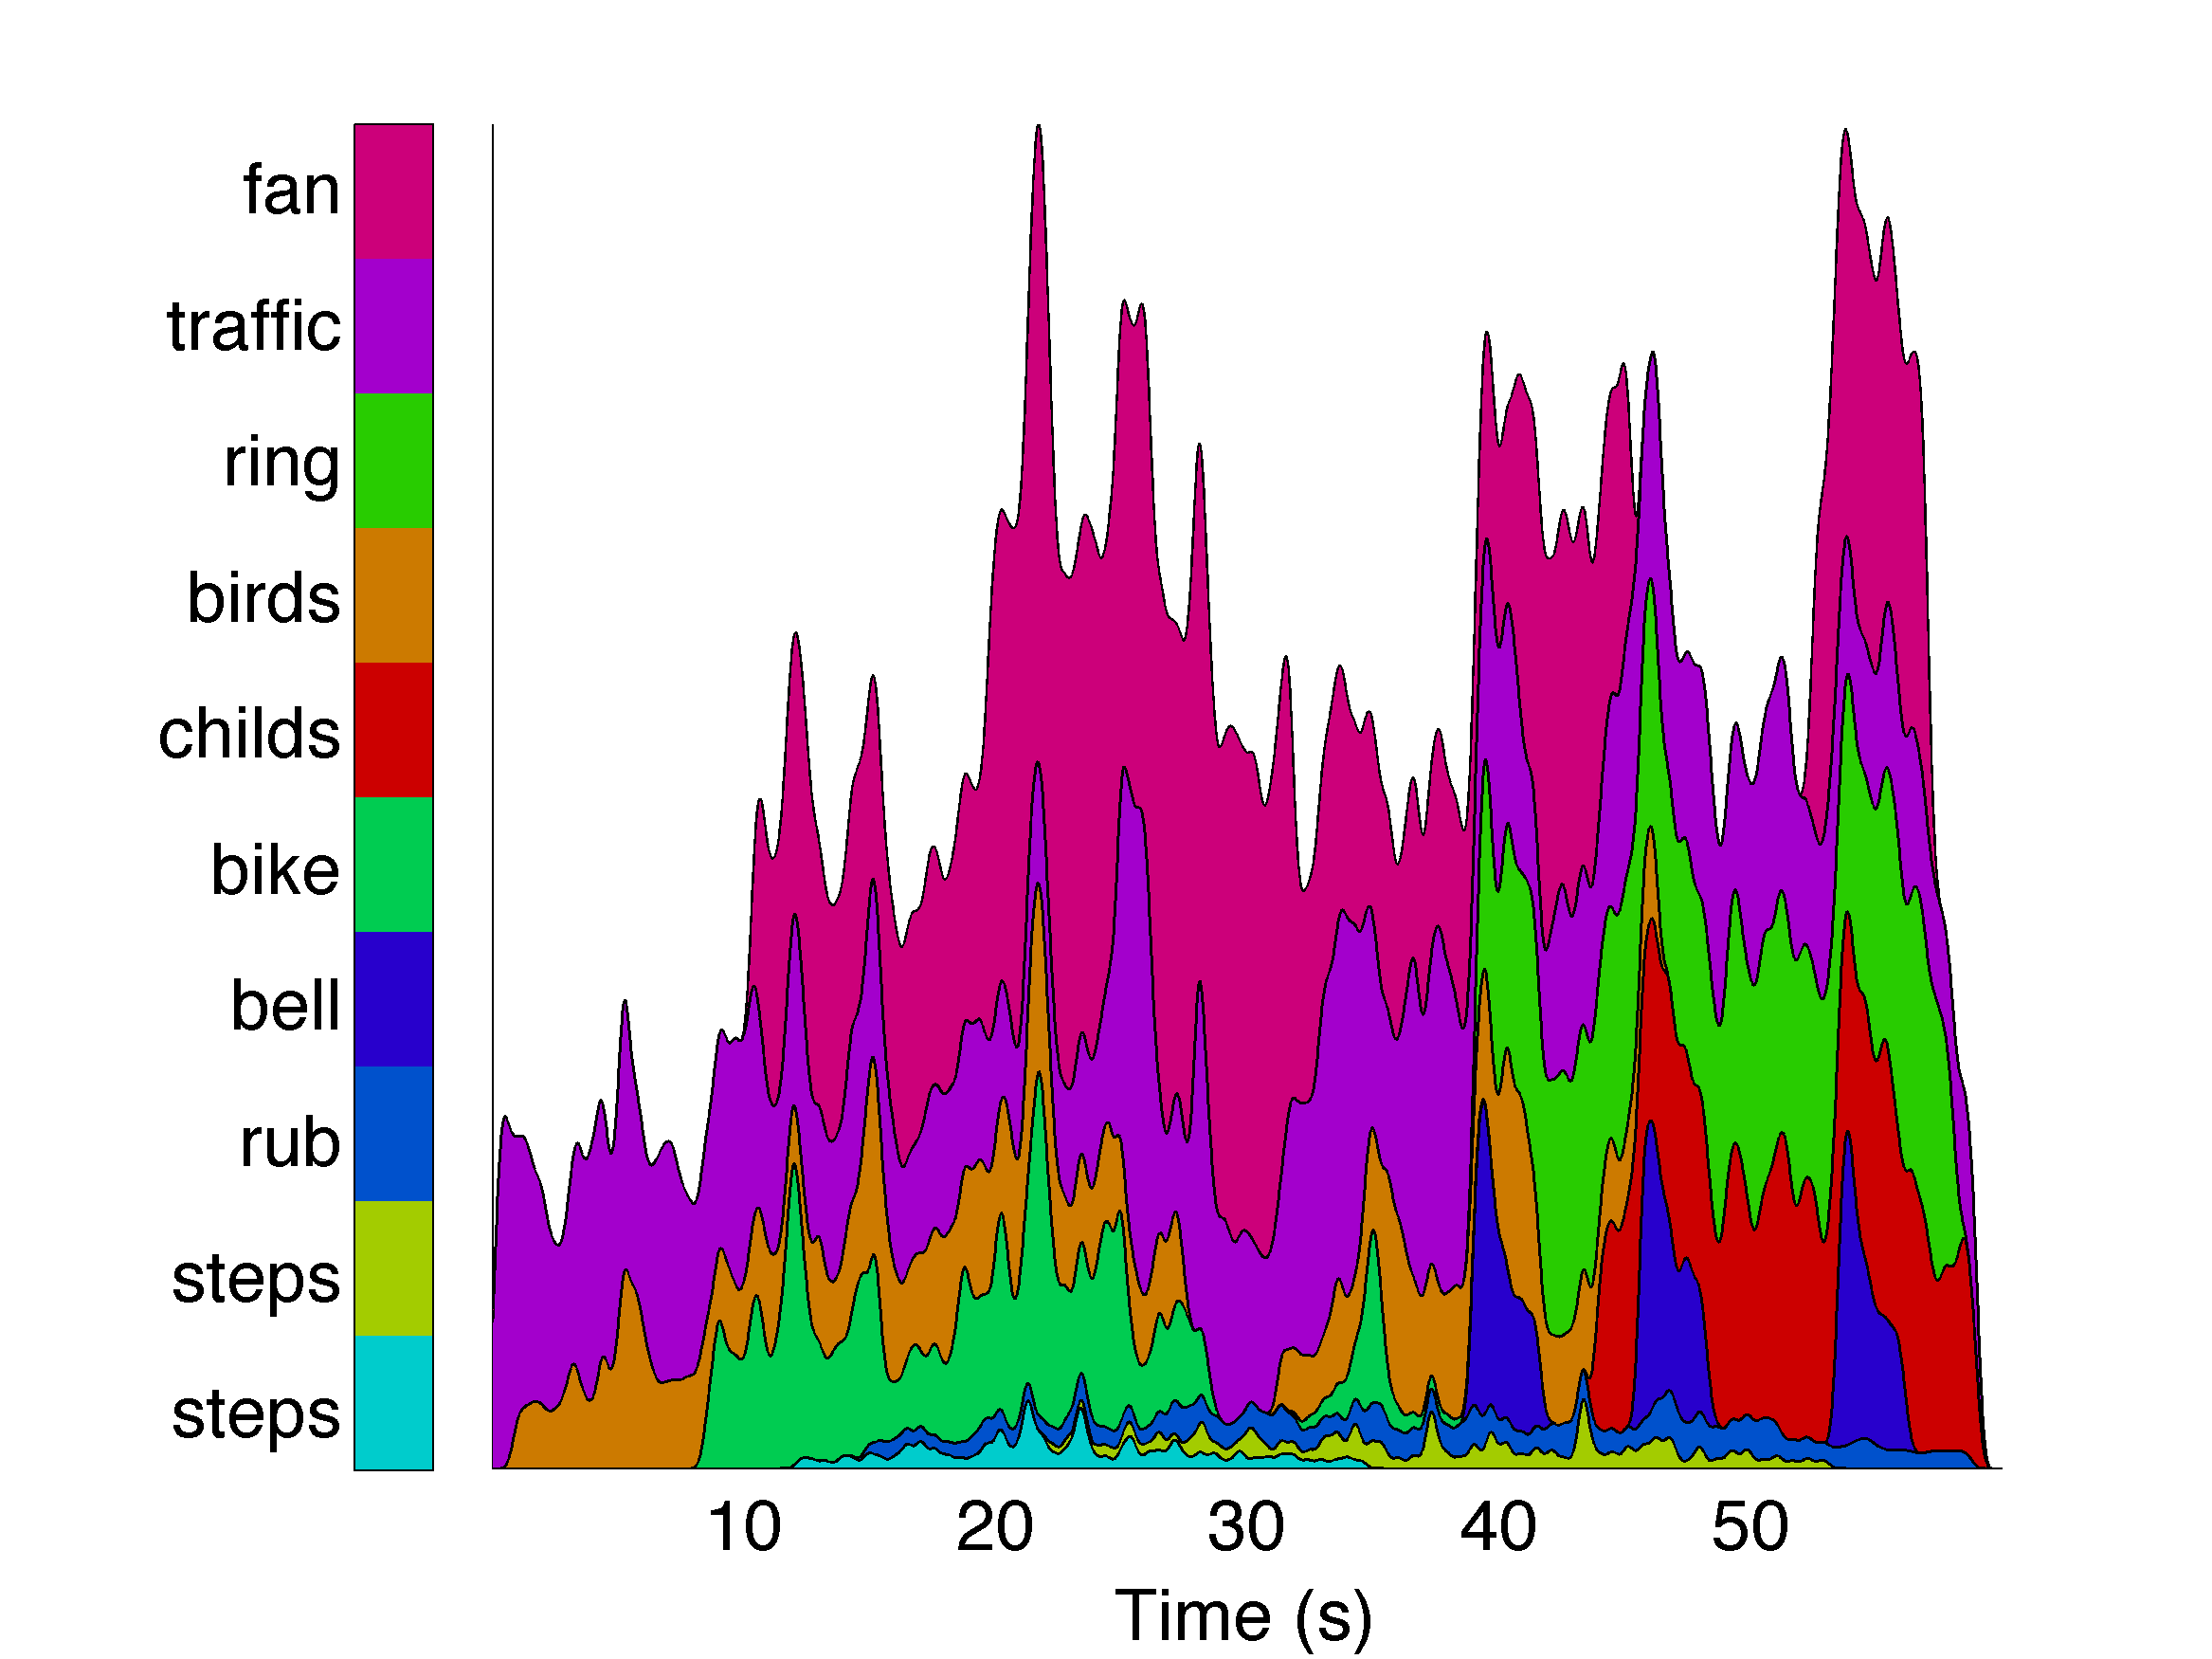
\includegraphics[width=\textwidth]{Multisource_smack}
\label{fig:smack_color}
\end{subfigure}
\begin{subfigure}[b]{.5\textwidth}
\caption{Gray scale display.}
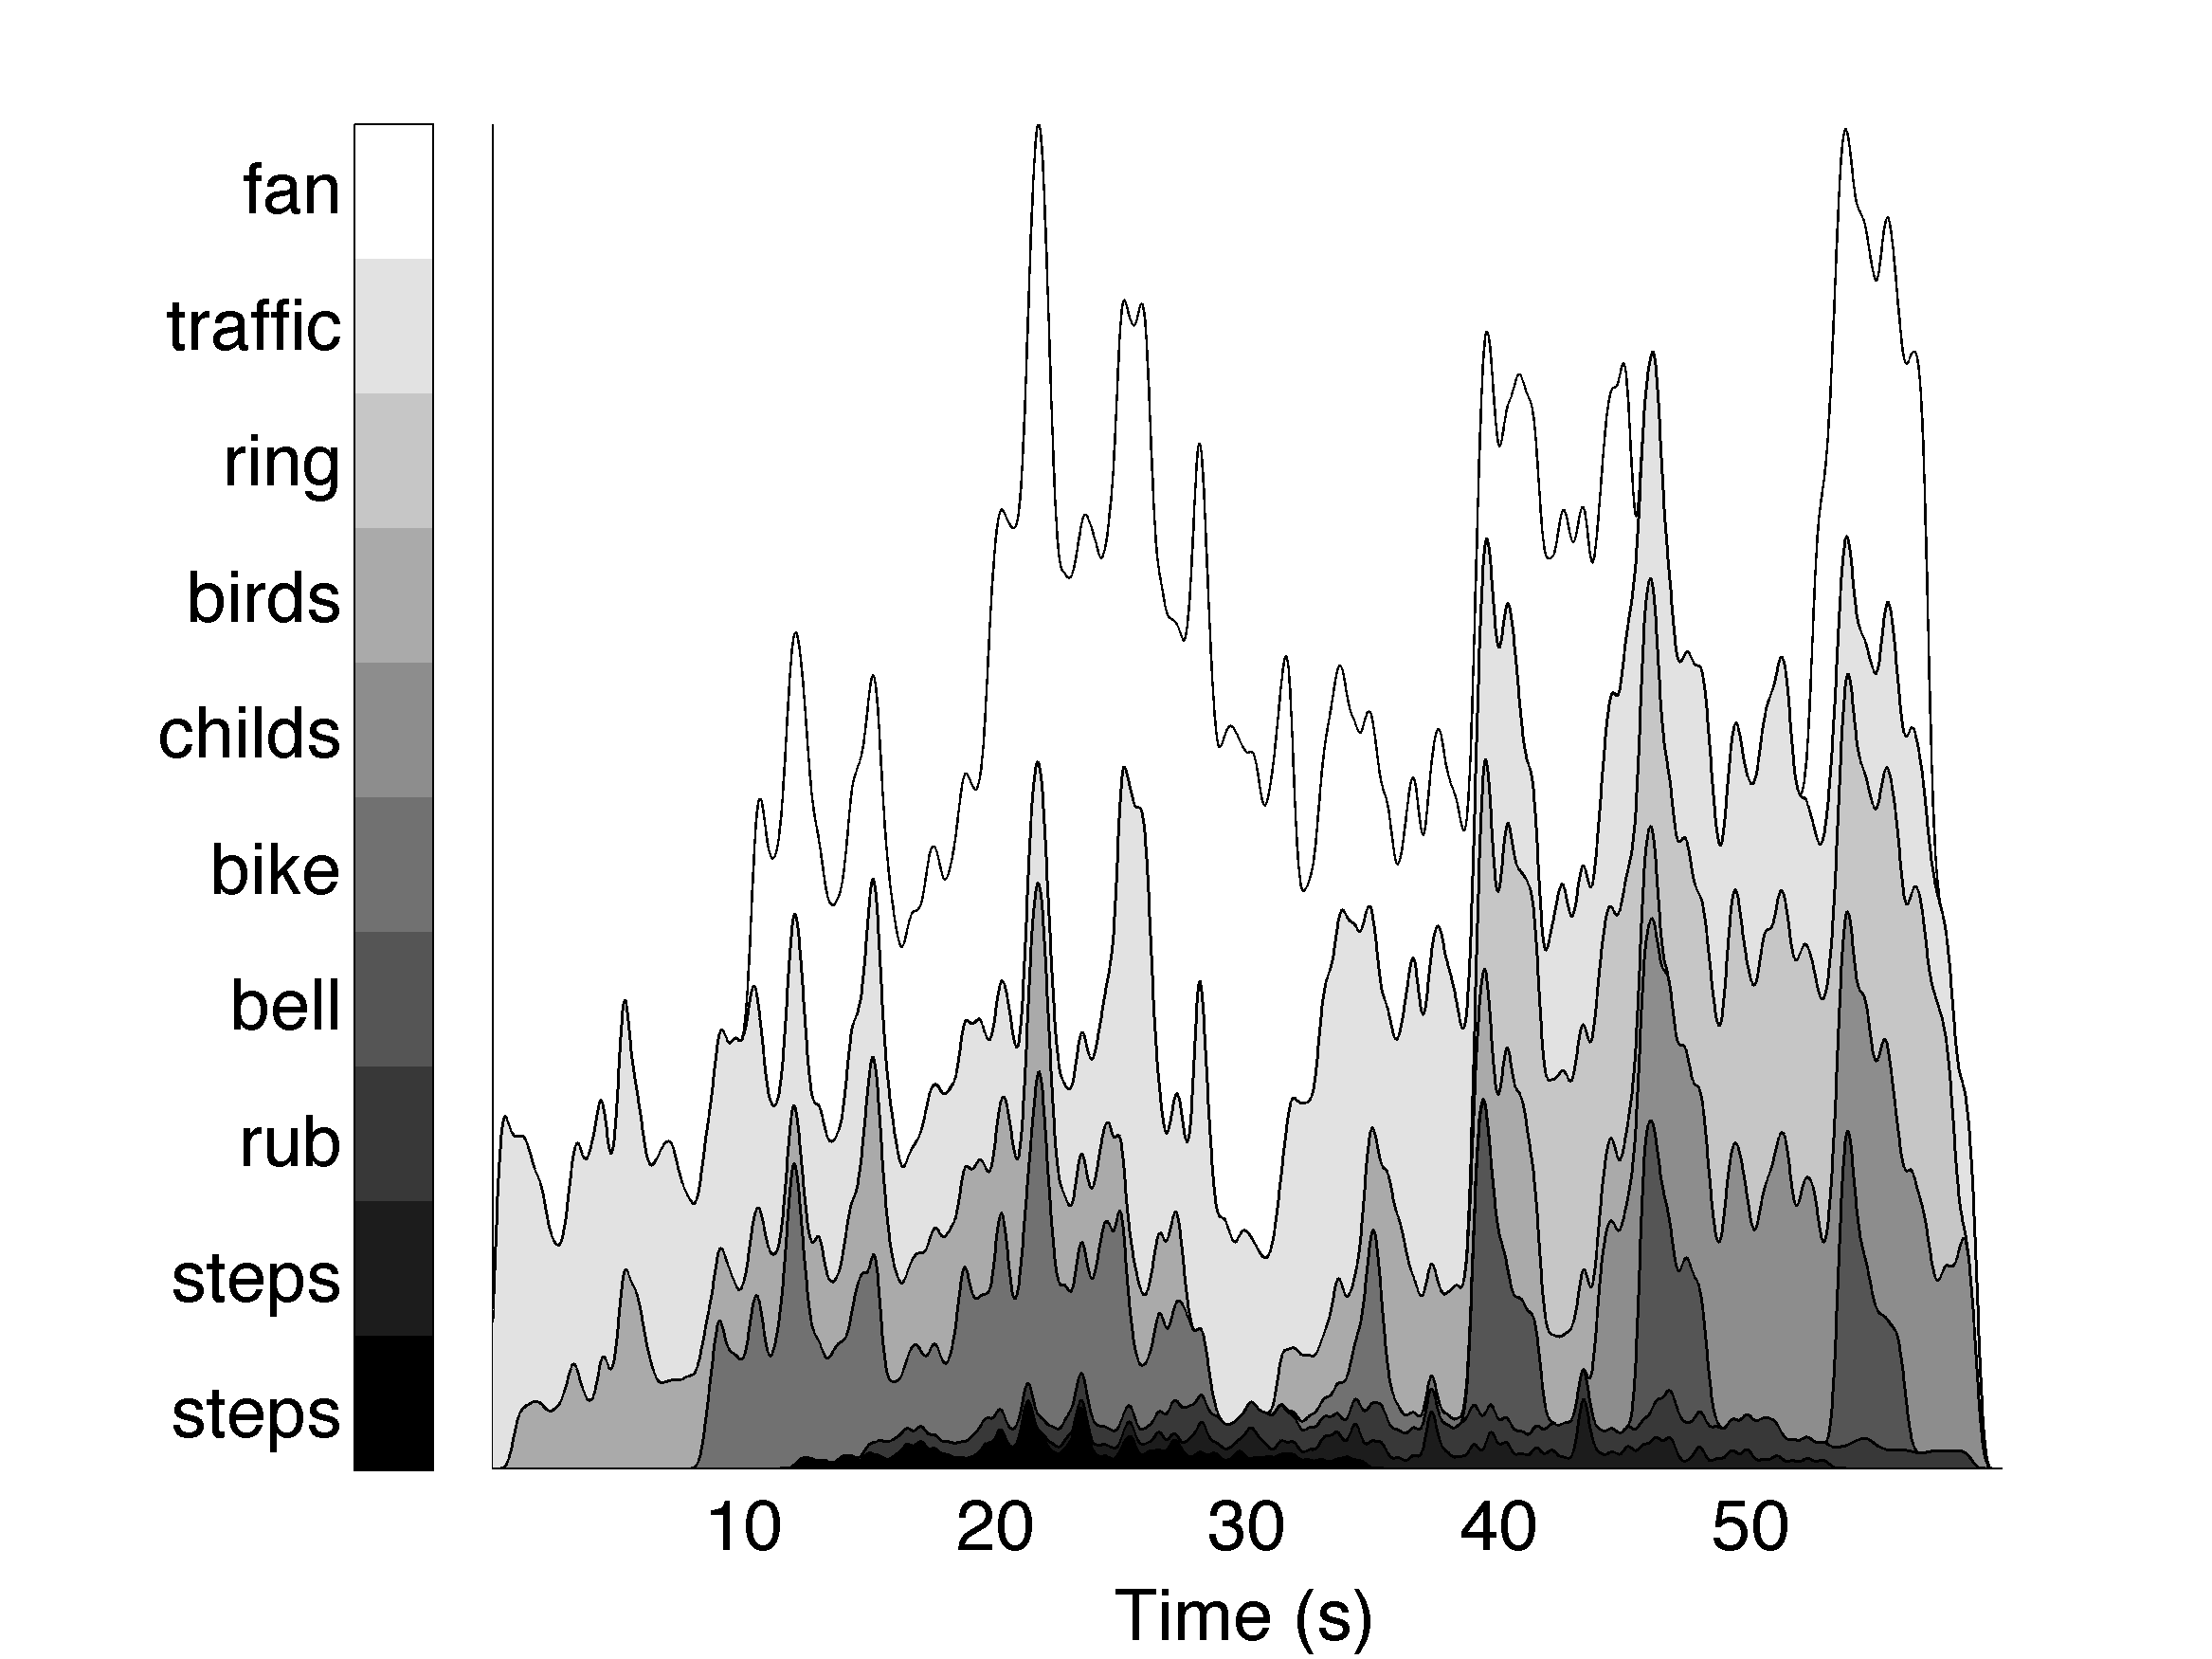
\includegraphics[width=\textwidth]{Multisource_smack_gray}
\label{fig:smack_gray}
\end{subfigure}
 \vspace{-20pt}
\caption{Sound Multiple stACK (SMACK) display of an environmental soundscape.}
\label{fig:smack}
 \vspace{-20pt}
\end{figure}


\section{Visualizing multi channel content (scack)}\label{sec:scack}

Another setting where such a style of display can be useful is to display multiple channels. On Figure \ref{fig:scack} is shown an arrangement of the 6 channels of a 5.1 setting. The color code is chosen in order to use hue to convey panning information and luminance to convey depth. The subwoofer is assigned to black as it is an omnidirectional source. In gray scale or black and white, the display is still legible due to the use of the vertical axis to convey panning information.
%, see respectively Figures \ref{fig:scack_gray} and \ref{fig:scack_bw}.

\begin{figure}[ht]
\begin{center}
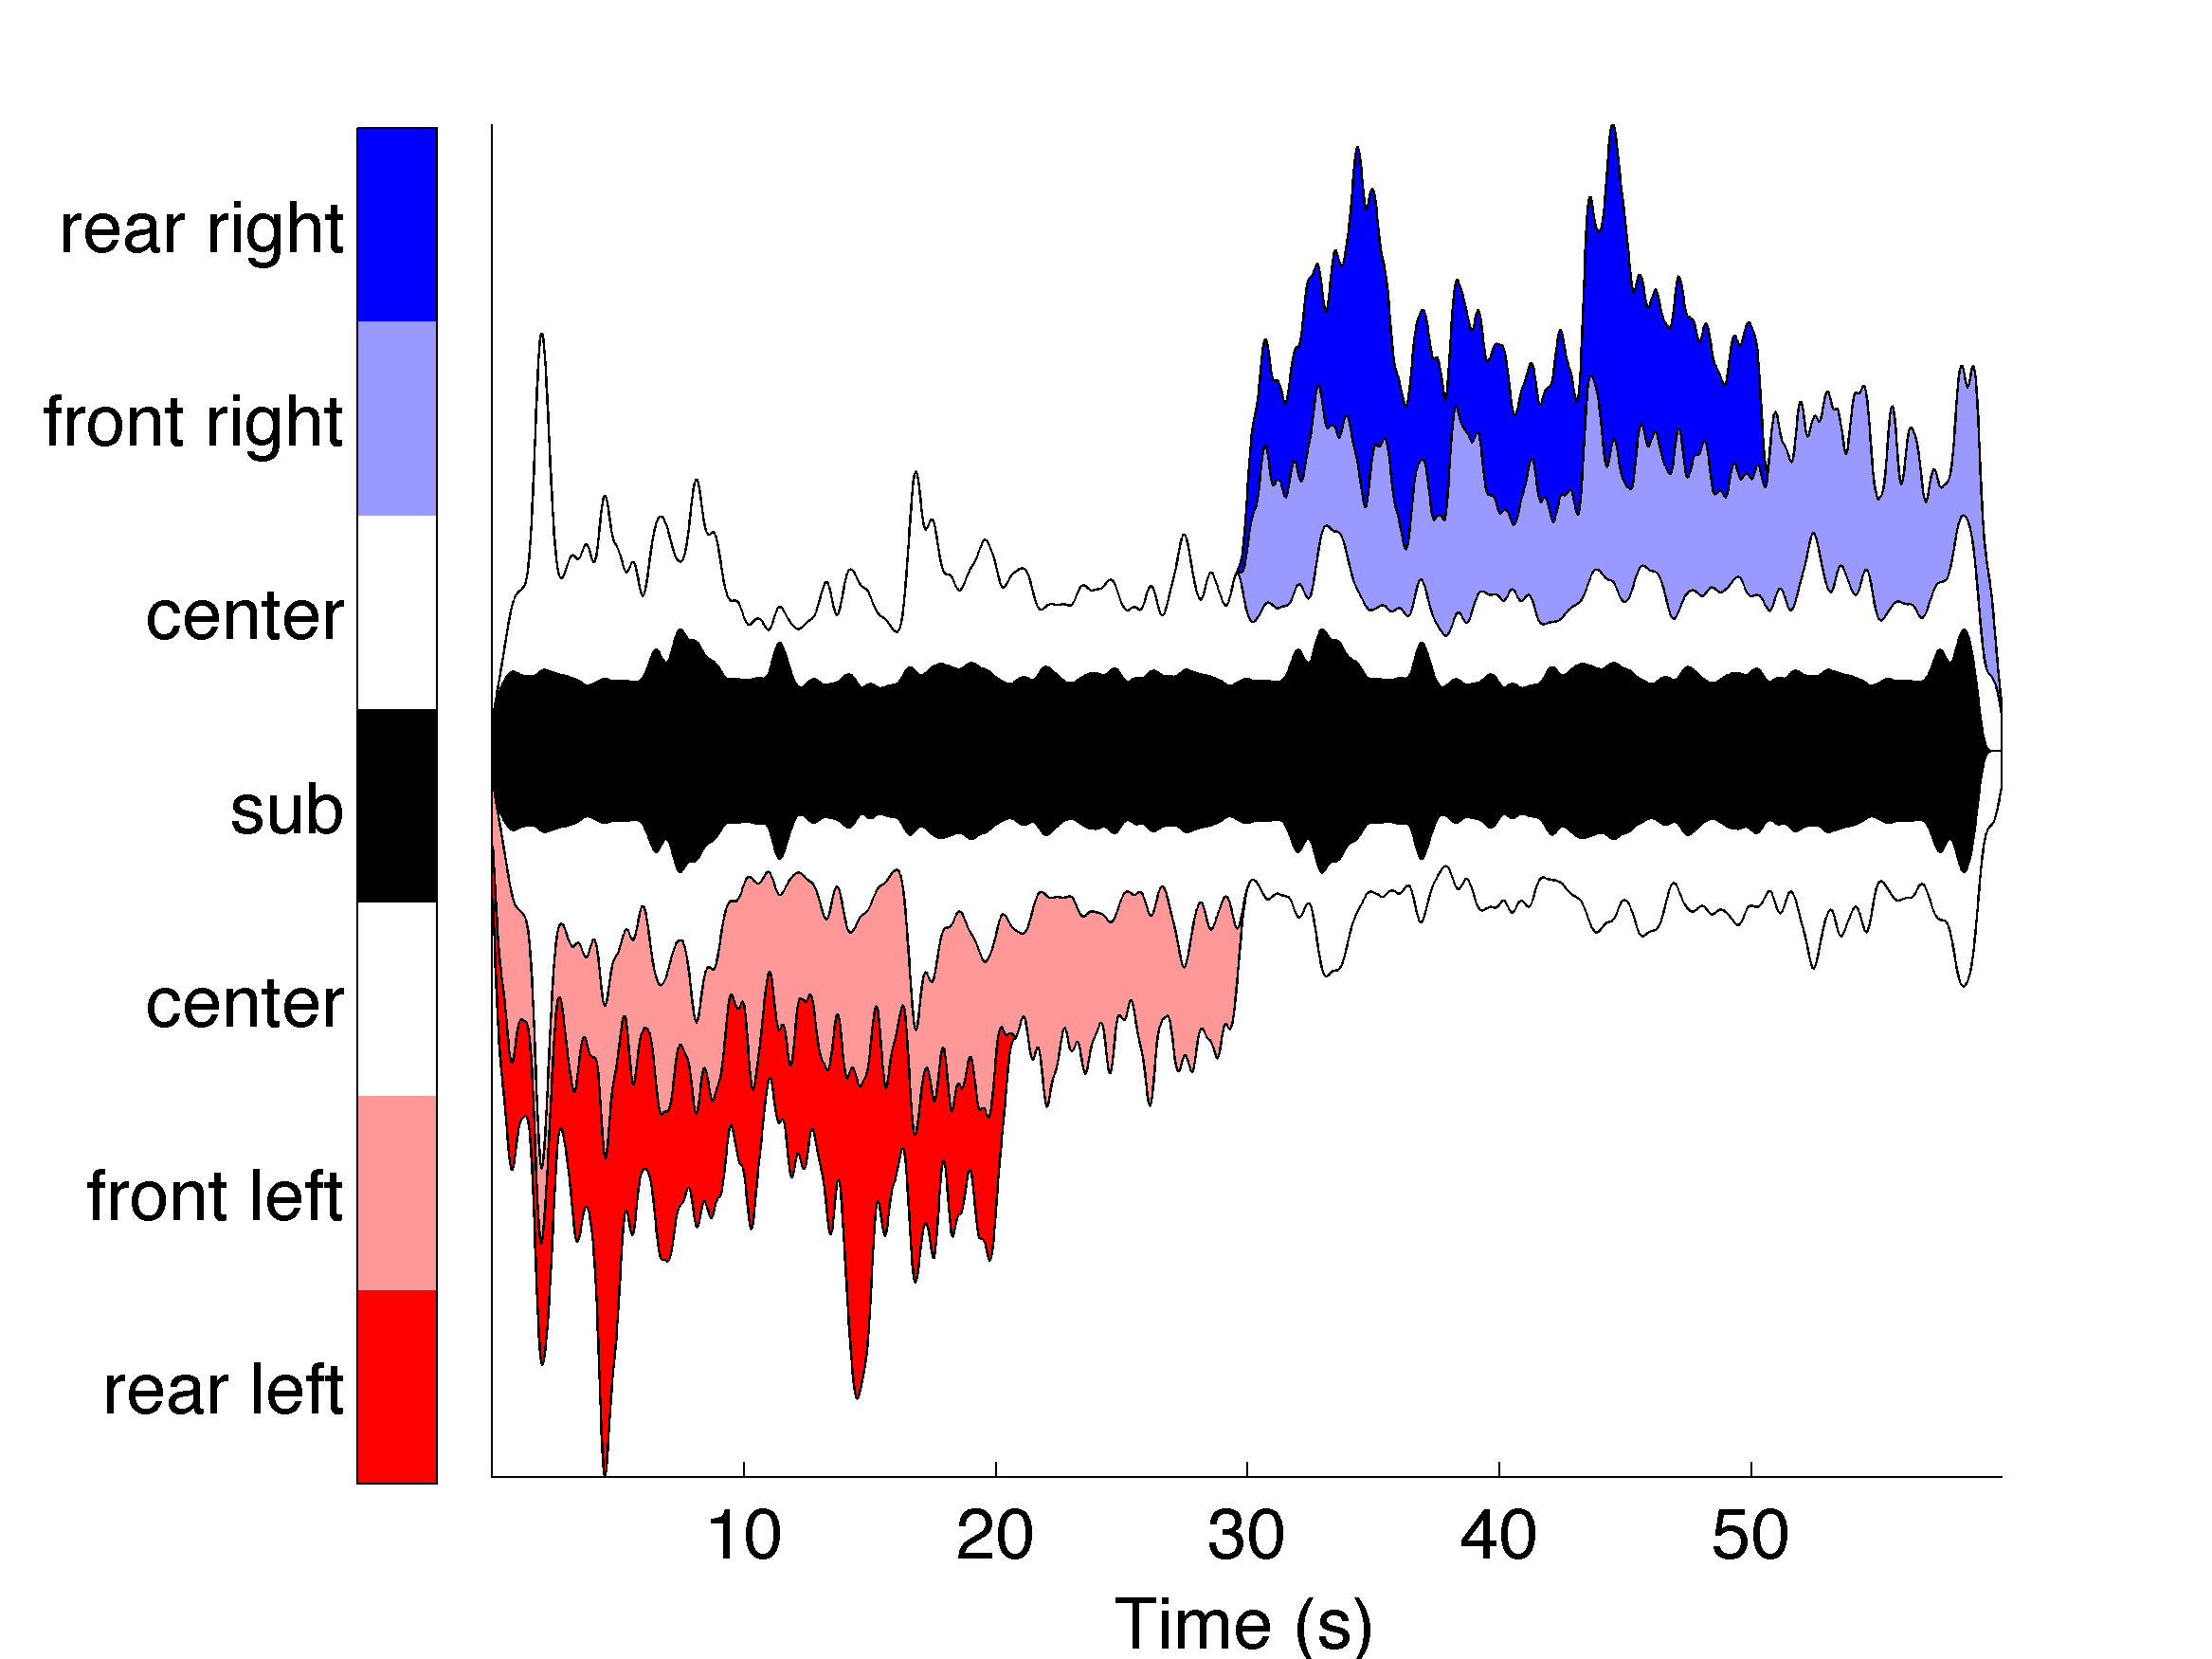
\includegraphics[width=.5\textwidth]{51SceneSynth_scack}
\caption{}
\label{fig:scack}
\end{center}
\end{figure}

%\begin{figure}[htbp]
%\begin{center}
%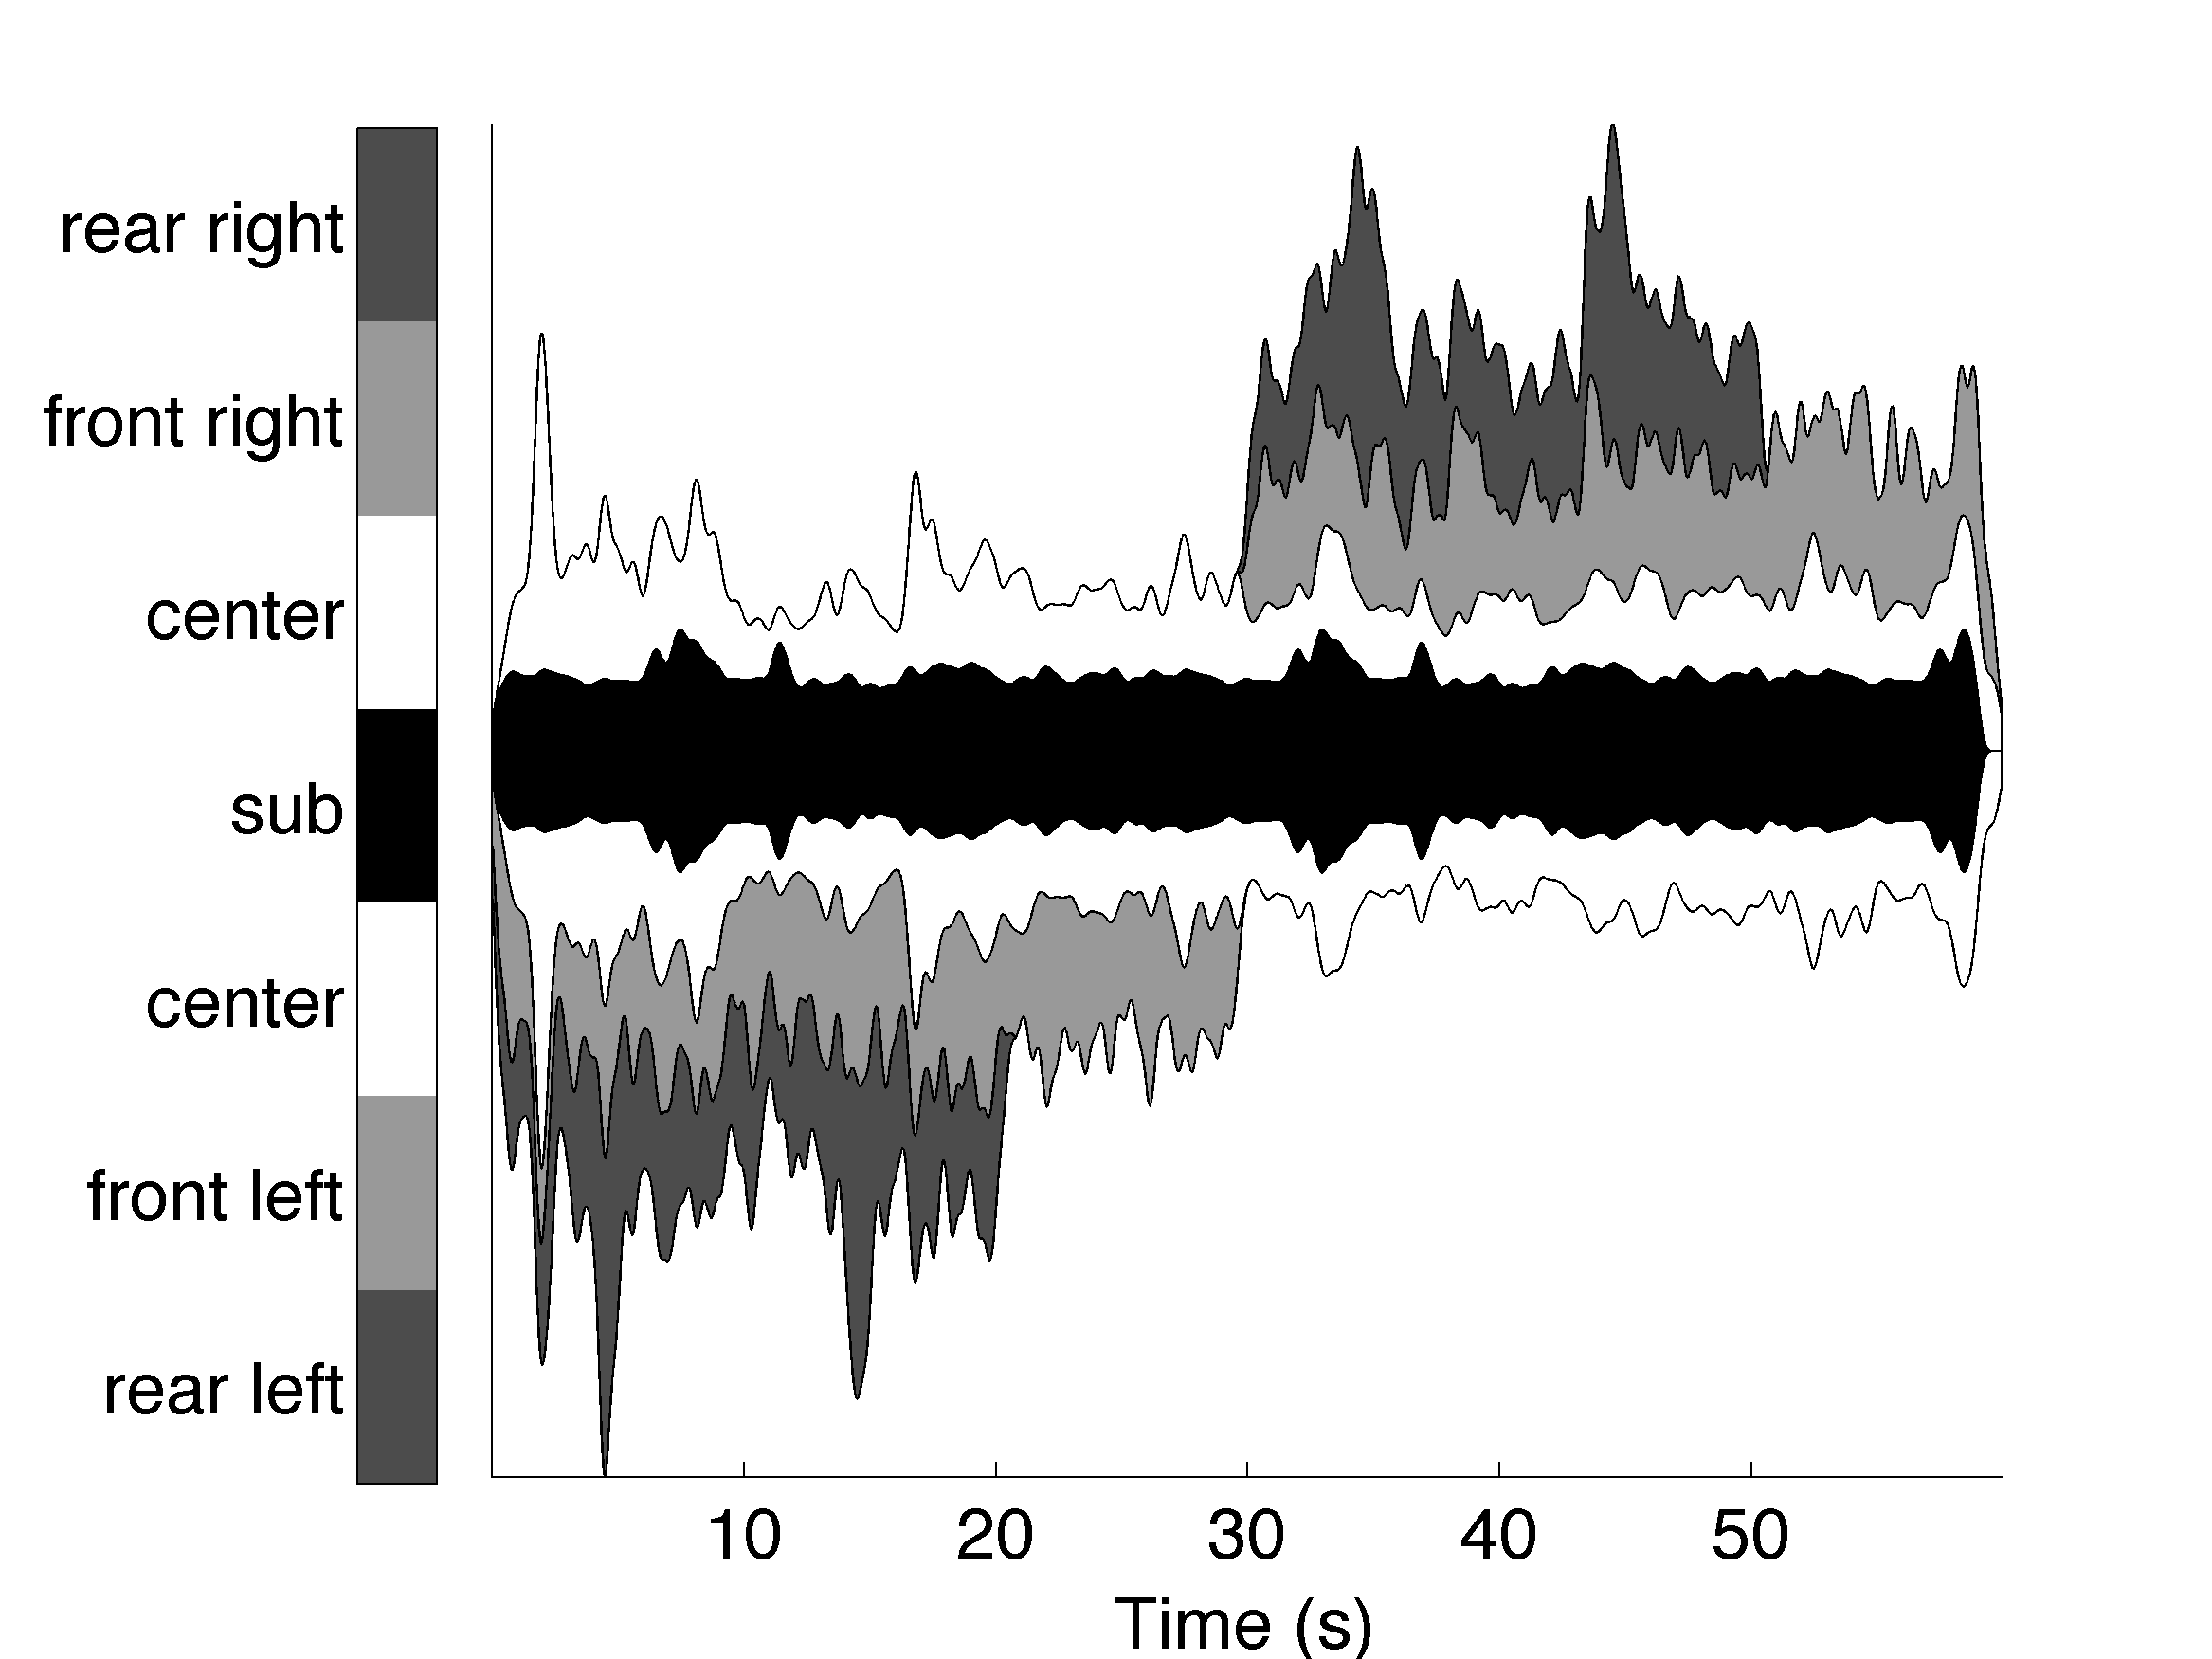
\includegraphics[width=.5\textwidth]{51SceneSynth_scack_gray}
%\caption{}
%\label{fig:scack_gray}
%\end{center}
%\end{figure}
%
%\begin{figure}[htbp]
%\begin{center}
%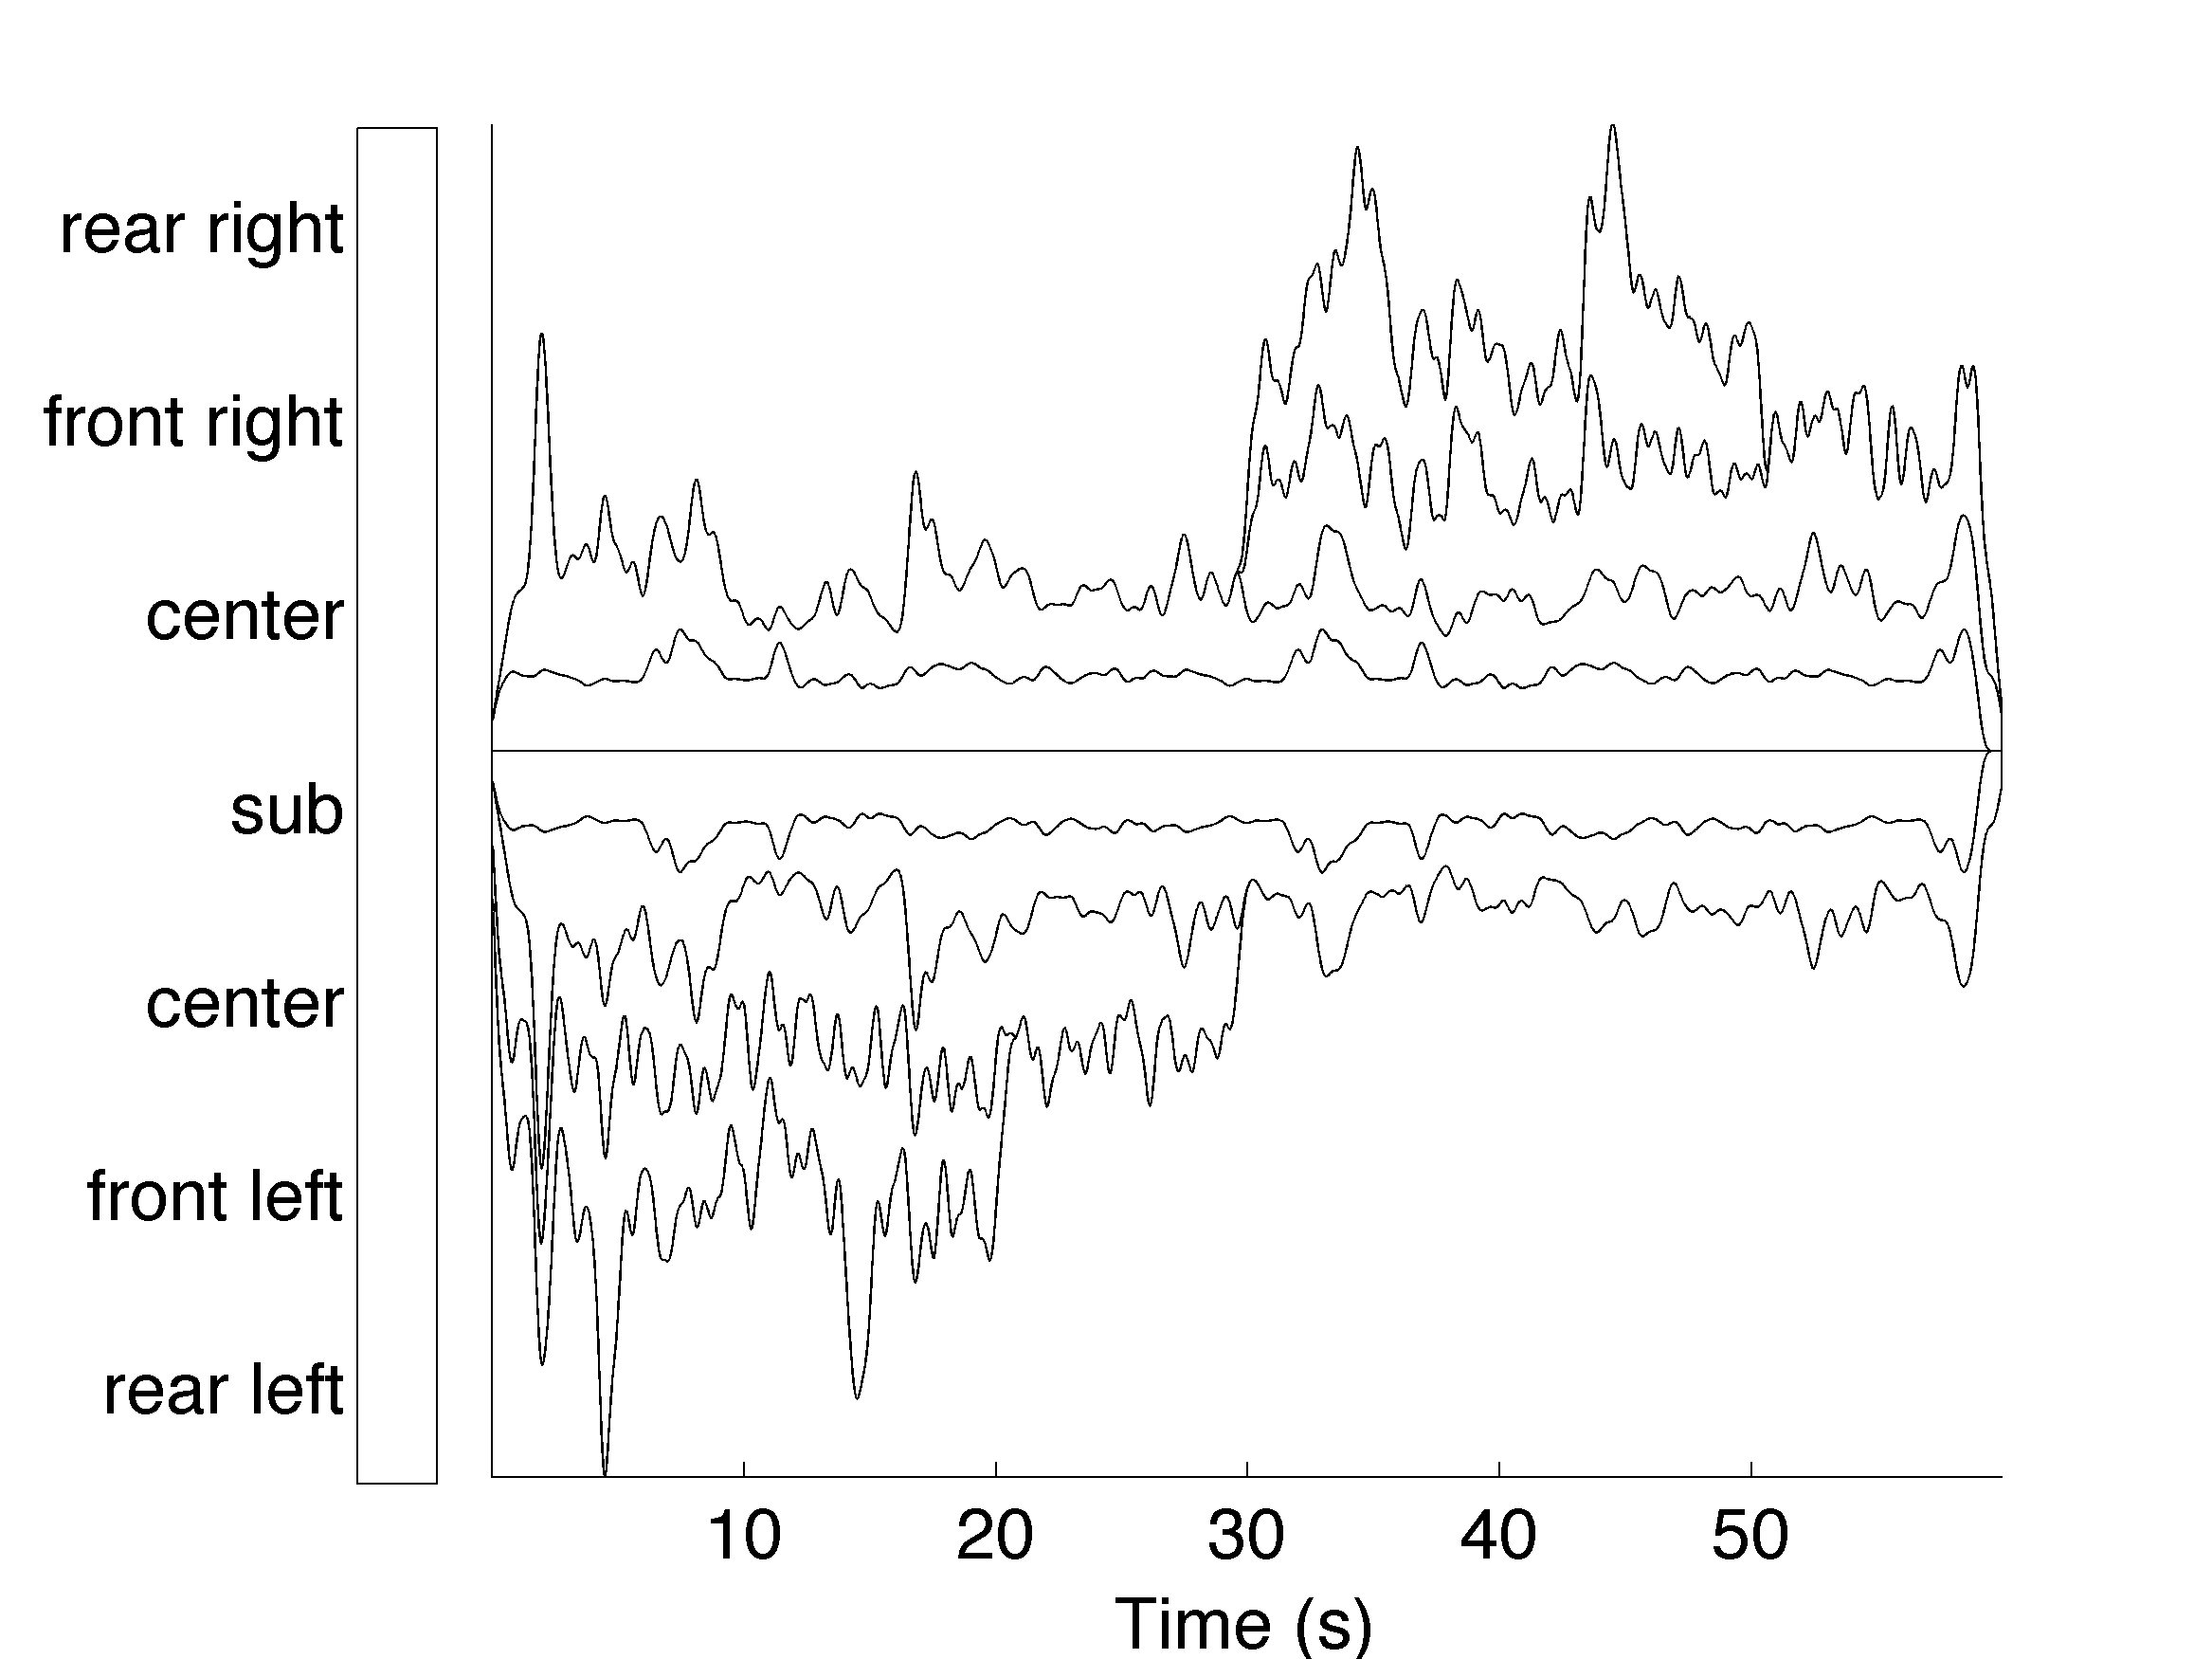
\includegraphics[width=.5\textwidth]{51SceneSynth_scack_bw}
%\caption{}
%\label{fig:scack_bw}
%\end{center}
%\end{figure}


\section{Visualizing melodic content}\label{sec:schack}

This display may also be used to represent the chroma, a feature widely used to describe musical signals. In our implementation, chroma is obtained by warping the spectral content of the signal into the well tempered western music scale of 12 semi-tones. % `wildly' used, haha -- ``Chromas gone wild''
%As for the SPACK (see \ref{sec:spack}) We use a 2D representation with time on the horizontal axis and energy on the vertical axis. 
In this display, termed Sound CHroma staCK (SCHACK), each chroma is described by a stacked layer of a carefully chosen color. % Mais si c'est vraiment 'wild', on peut aussi l'appeler SHAG

To set a meaningful color map, we got our inspiration from the color-tonality association made by Scriabine \cite{Galeyev2001}. Scriabine was a synesthete who extensively experimented the relationship between sounds and colors. He made an color-tonality association in which two tones which are in close proximity in the cycle of fifth are represented which similar colors. Considering that Scriabine's choice of colors was subjective, and the associations he made was between tones and colors and not notes and colors\cite{Galeyev2001}. As a chroma is more related to the notion of note than the notion of tone, we chose a more common color set while maintaining the color mapping based on the cycle of fifths. \\
  
%% Je ne comprends pas ``ton'' ici. Si tu veux dire ``gamme'', c'est plutot ``scale''
To represent the 12 notes of the scale, we use 12 colors in a HSV color space (\textit{Hue}, \textit{Saturation}, \textit{Value}),  each of them having the same \textit{Saturation} and \textit{Value} and differ only in their \textit{Hue}.  The 12 colors of our HSV space are mapped onto the 12 notes of the musical scale ordered in a cycle of fifths, see Figure \ref{fig:cycleQuinte}. Doing so ensures that two consecutive chroma (\textit{ie.} semi-tones in that case) are represented with distinct colors, which are helpful for a stack based representation. Furthermore this color-map is  adapted to illustrate both unique notes and chords.

If we consider a single note, the color-map allows us to represent the first four partials of the note, which are the octave, the Pythagorean  fifth (which can be considered as the perfect fifth of the fundamental frequency  to within a few comma), and double octave of the fundamental frequency, with similar colors having regards to their saturation. All the others partials are represented with distinct colors (see figure \ref{fig:fluteGammeMonoNorm_schack}). 

If we consider a chord, the color-map allows us to represent two "consonant" notes (fifth, fourth, major second intervals) with two closed colors  in term of saturation and two "dissonant" notes (Tritone: \textit{Diabolus in musica} or minor second intervals) with well distinct colors, in the case that of the spectral energy is contained in the fundamental frequency. Those notions of "consonant" and "dissonant" have a significant relevance to the Western tonal music theory. Third and sixth intervals may be also considered "consonant" interval, but as the color mapping is based on the cycle of fifths, third and sixth intervals are not represented with particular colors associations. 

Let us consider a musical example. Figure \ref{fig:duoFluteMono_schack} show the schack representation of the beginning of a flute \textit{Duett} composed by Georg Philipp Telemann (see figure \ref{fig:telemann} for the score). The envelop of the stacked layers clearly illustrate that 1) the amplitude is modulated and  2) four notes (\textit{F}) are played with more intensity than the other notes. The color map allows us to distinguish the third first notes (\textit{B-flat} \textit{D} \textit{E-flat}) by identifying the broader layers, as most spectral energy is concentrated on their fundamental frequency and their first partial (octave). We can see that the \textit{B-flat} is maintained during the notes \textit{D} \textit{E-flat} as the thickness of the layer corresponding to  \textit{B-flat} remains important.  As the first three notes are relatively far from each others in the cycle of fifths, they are represented with distinct colors. For the fourth note (\textit{F}), the fact that the layers corresponding to the two adjacent semi tones (\textit{E-flat} and \textit{F-sharp}) are presents may be due to a lack of selectivity in the frequency analysis.
% (VOIR AVEC MATHIEU POURQUOI ON A CET EFFET DE DEBORDEMENT SUR LES SEMI TONS ADJACENTS: largeur du pic). 
For all the notes (\textit{F}), we can see that the amplitude of the third partials (Pythagorean  fifth, which would correspond to the note \textit{C}) is important. Every time the note \textit{F} is played, the red layer is broader. \\

Considering the first chord (\textit{E-flat}/\textit{F}) and the last chords (\textit{A}/\textit{F}), we can see that le layer of \textit{E-flat} is more important for the first chord (\textit{E-flat}/\textit{F}) than it is for the second chord (\textit{A}/\textit{F}), in which the layer of \textit{A} is broader.  \\


\begin{figure}[t]
\centering
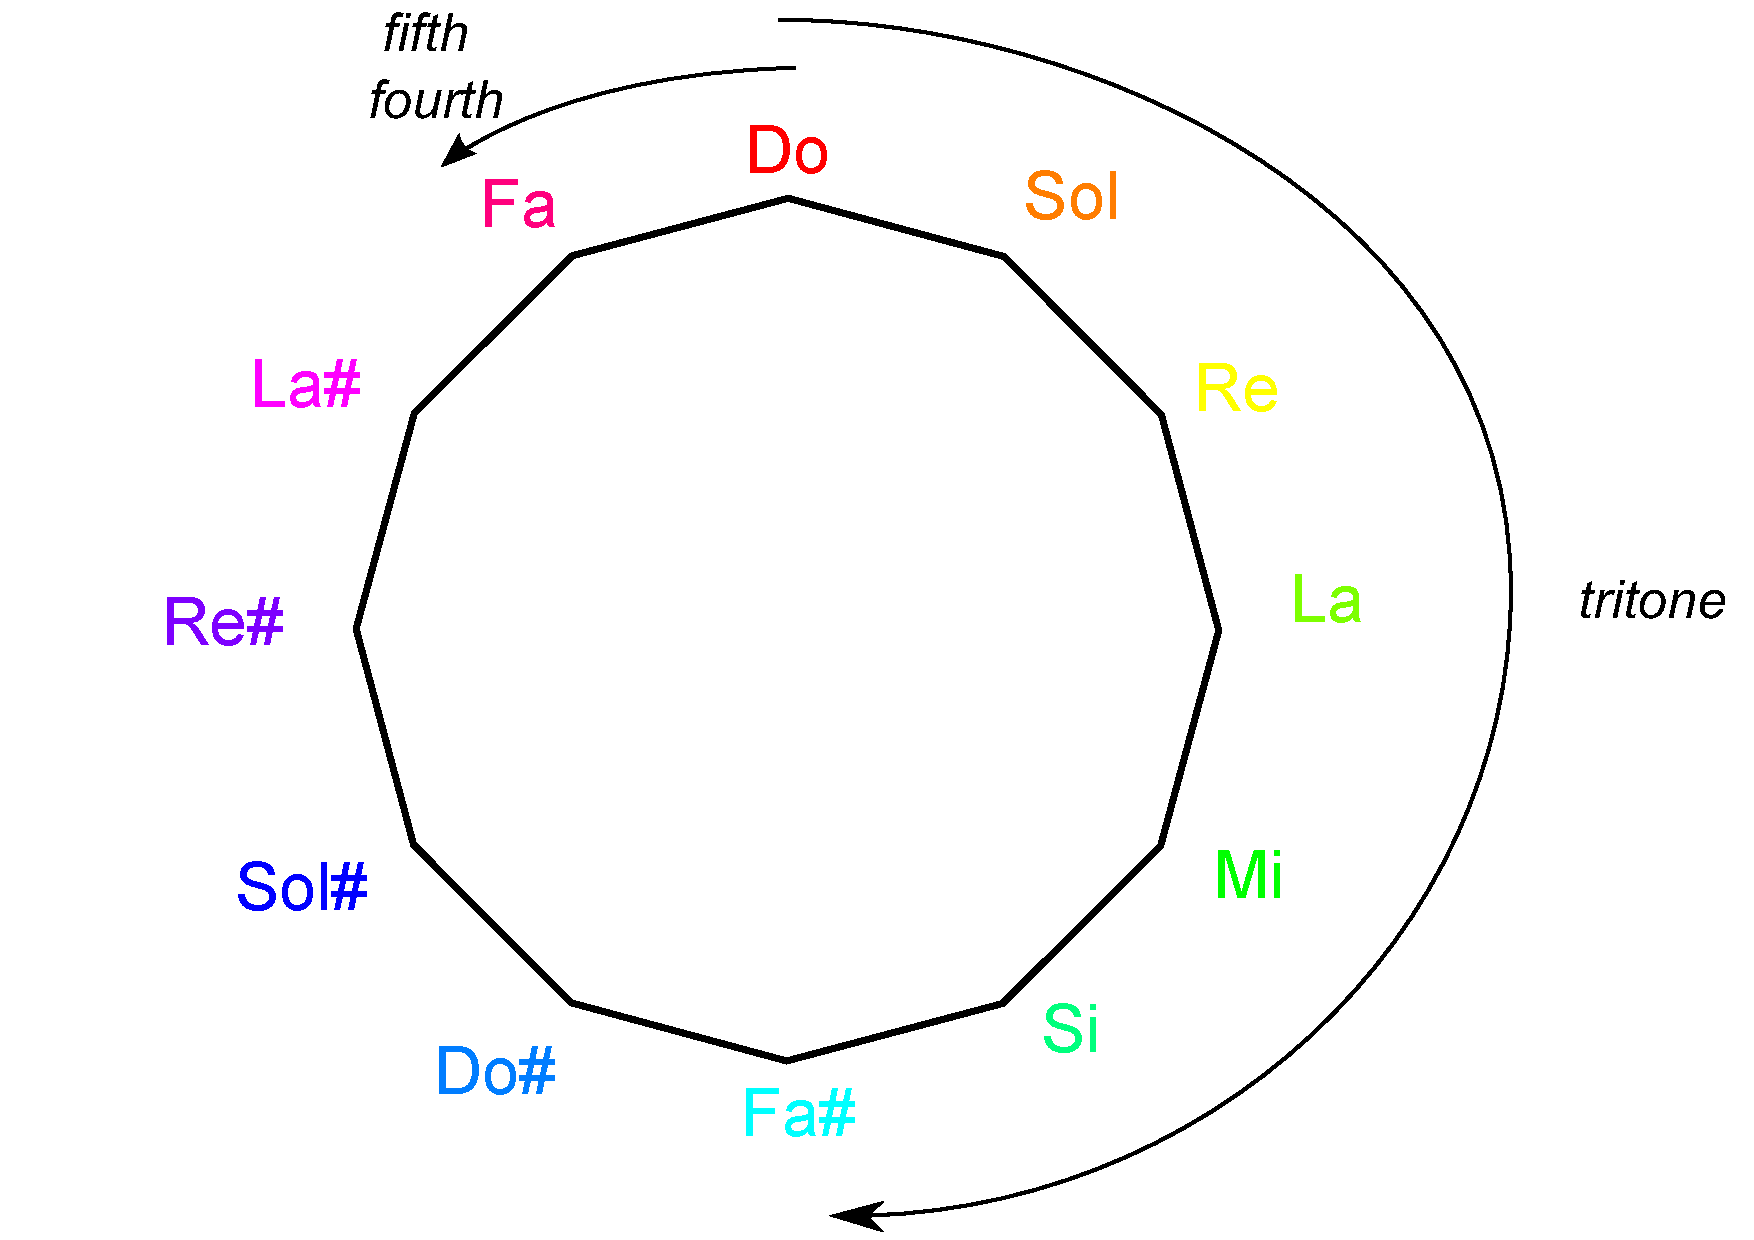
\includegraphics[width=.5\textwidth]{cycleQuinte.pdf}
\caption{Proposed mapping between HSV color space and the notes ordered in a cycle of fifths.}
\label{fig:cycleQuinte}
\end{figure} 


\begin{figure}[t]
\centering
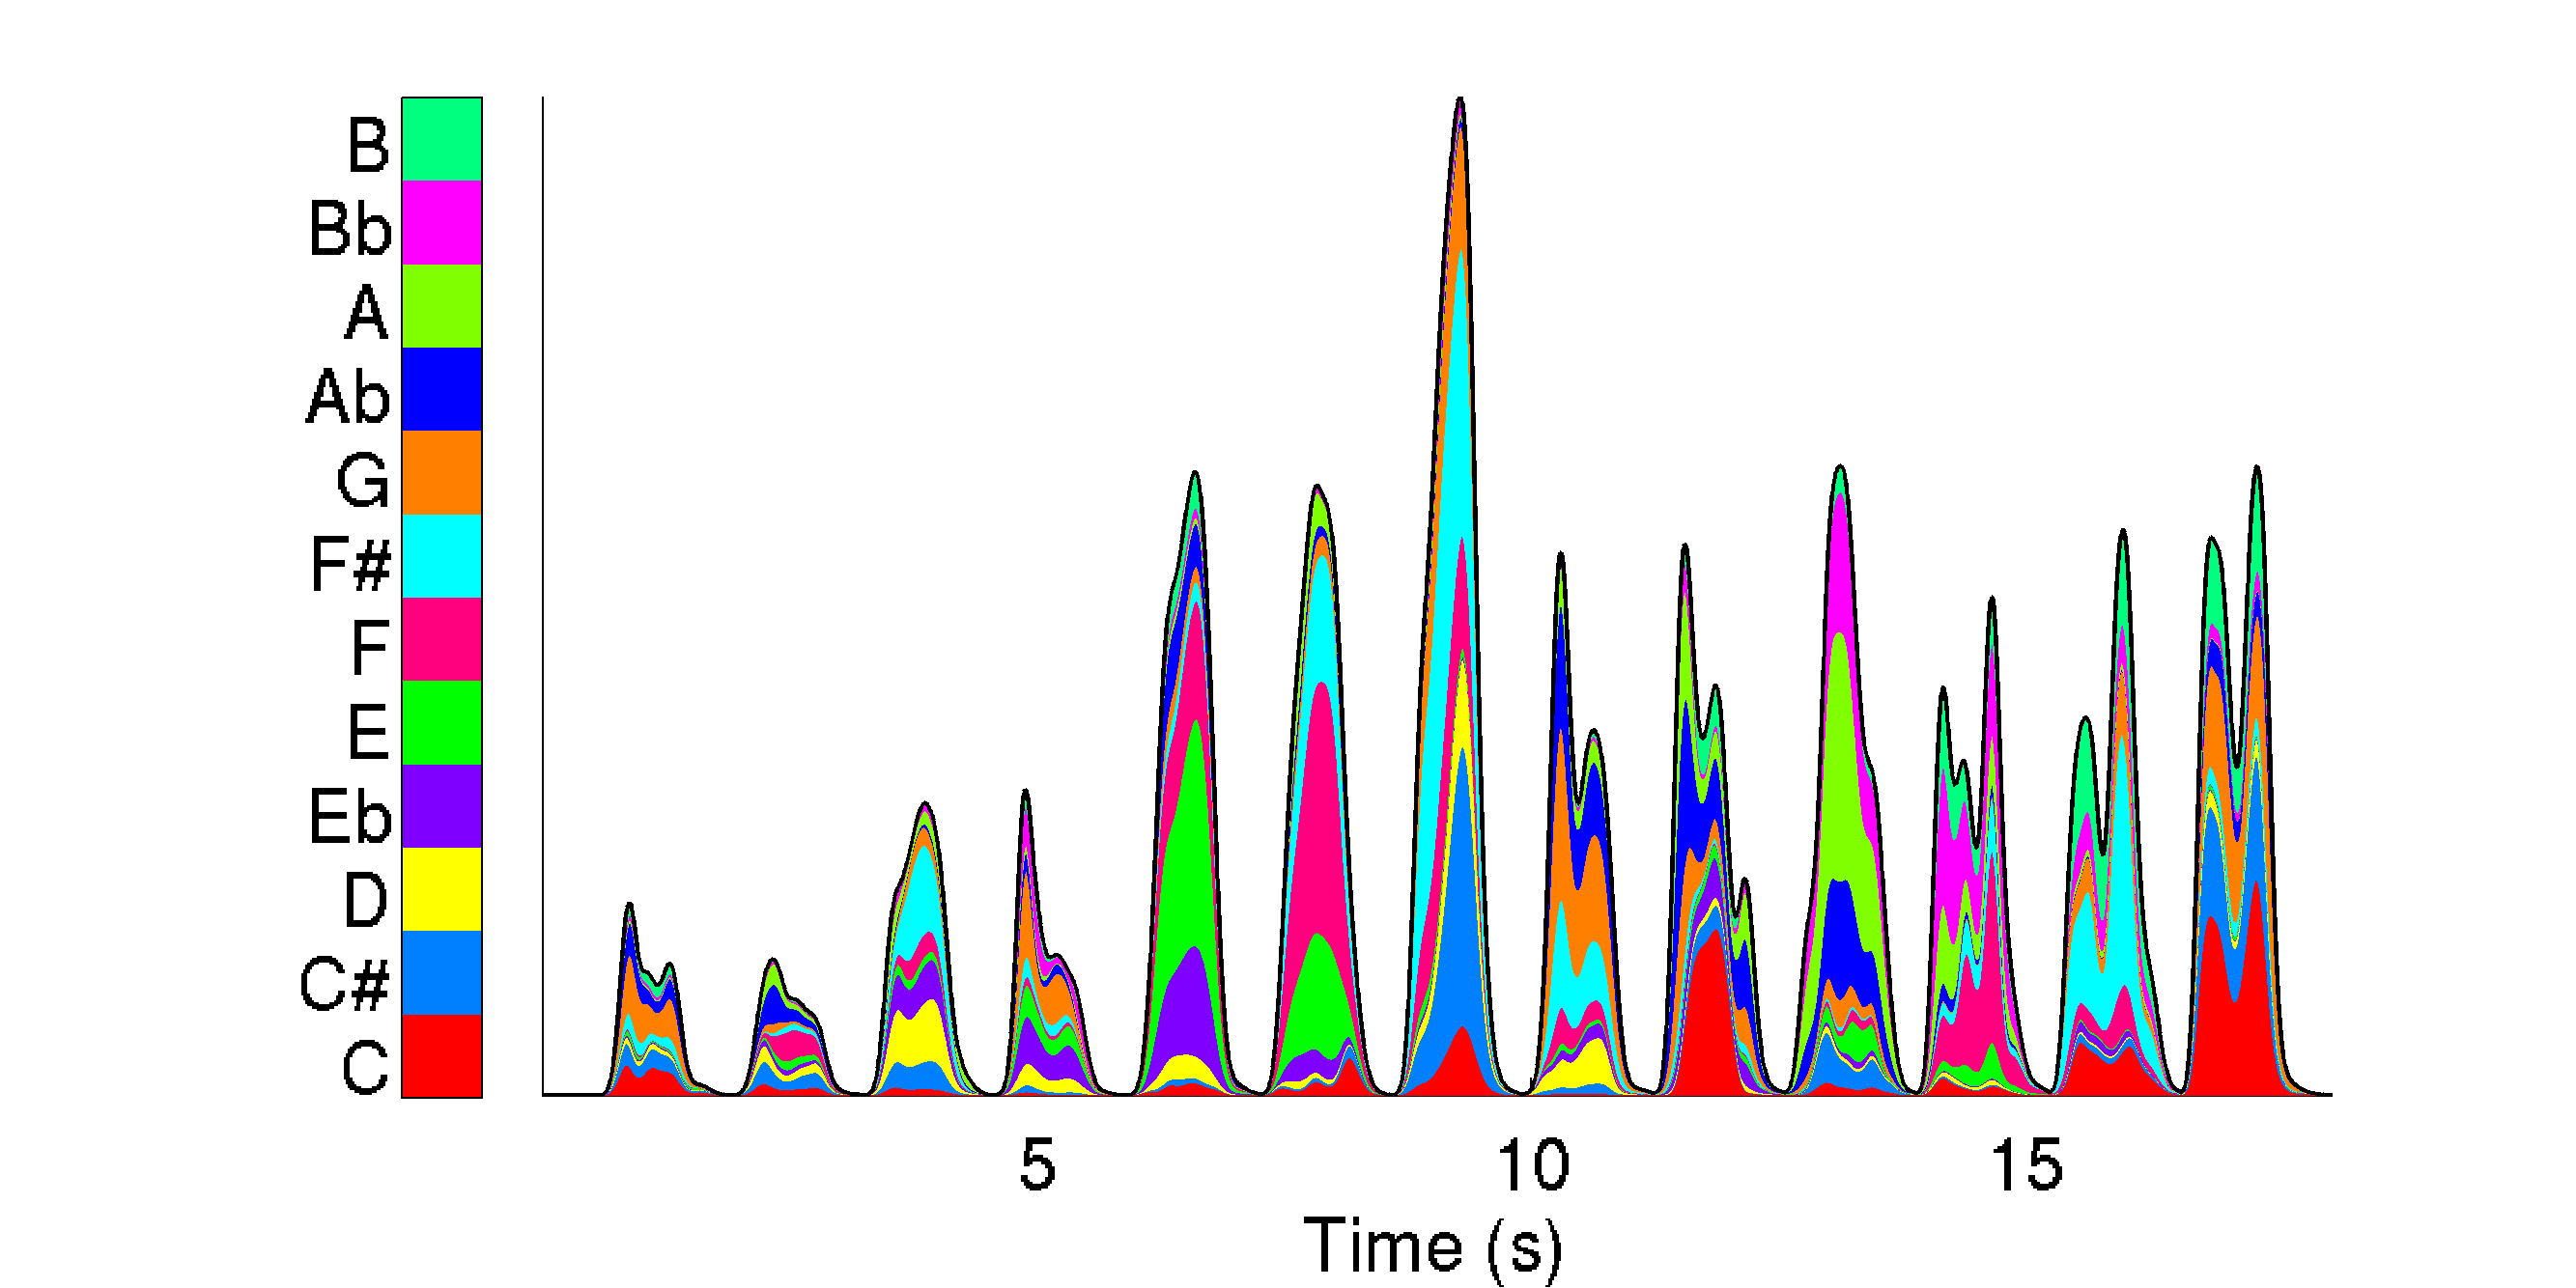
\includegraphics[width=.5\textwidth]{fluteGammeMonoNorm_schack}
\caption{Sound CHroma stACK (SCHACK) representation of a full musical scale of 12 semi-tones played by a flute.}
\label{fig:fluteGammeMonoNorm_schack}
\end{figure} 

\section{Discussion}\label{sec:discussion}

We introduced in this paper an interesting set of displays. For mono channel data, the spectral and chromatic displays allows the user to display frequency related information on a time / energy plane, thus nicely conveying information about the variation of energy trough time. For multi sources or multichannel data, the proposed displays allow the user to display a large amount of information on a single graph.

Even though the displays are designed to be meaningful in a large set of applications, some settings are application dependent. Whether or not a compression shall be applied typically depends on the type of data to be analyzed. For speech data, it leads to much better display, whereas for many environmental sounds it may degrade the timing information. An horizontal smoothing using a gaussian kernel is applied in order to reduce high frequency variations that would blur the visual display. The size of the kernel typically depends on the duration of the audio but also on the style of display. 

\section{Acknowledgments}

The implementation provided is based on the rastamat toolbox written by Dan Ellis. Research project partly funded by ANR-11-JS03-005-01.

\bibliographystyle{plain}
\bibliography{bib}



\begin{figure*}
 \centering
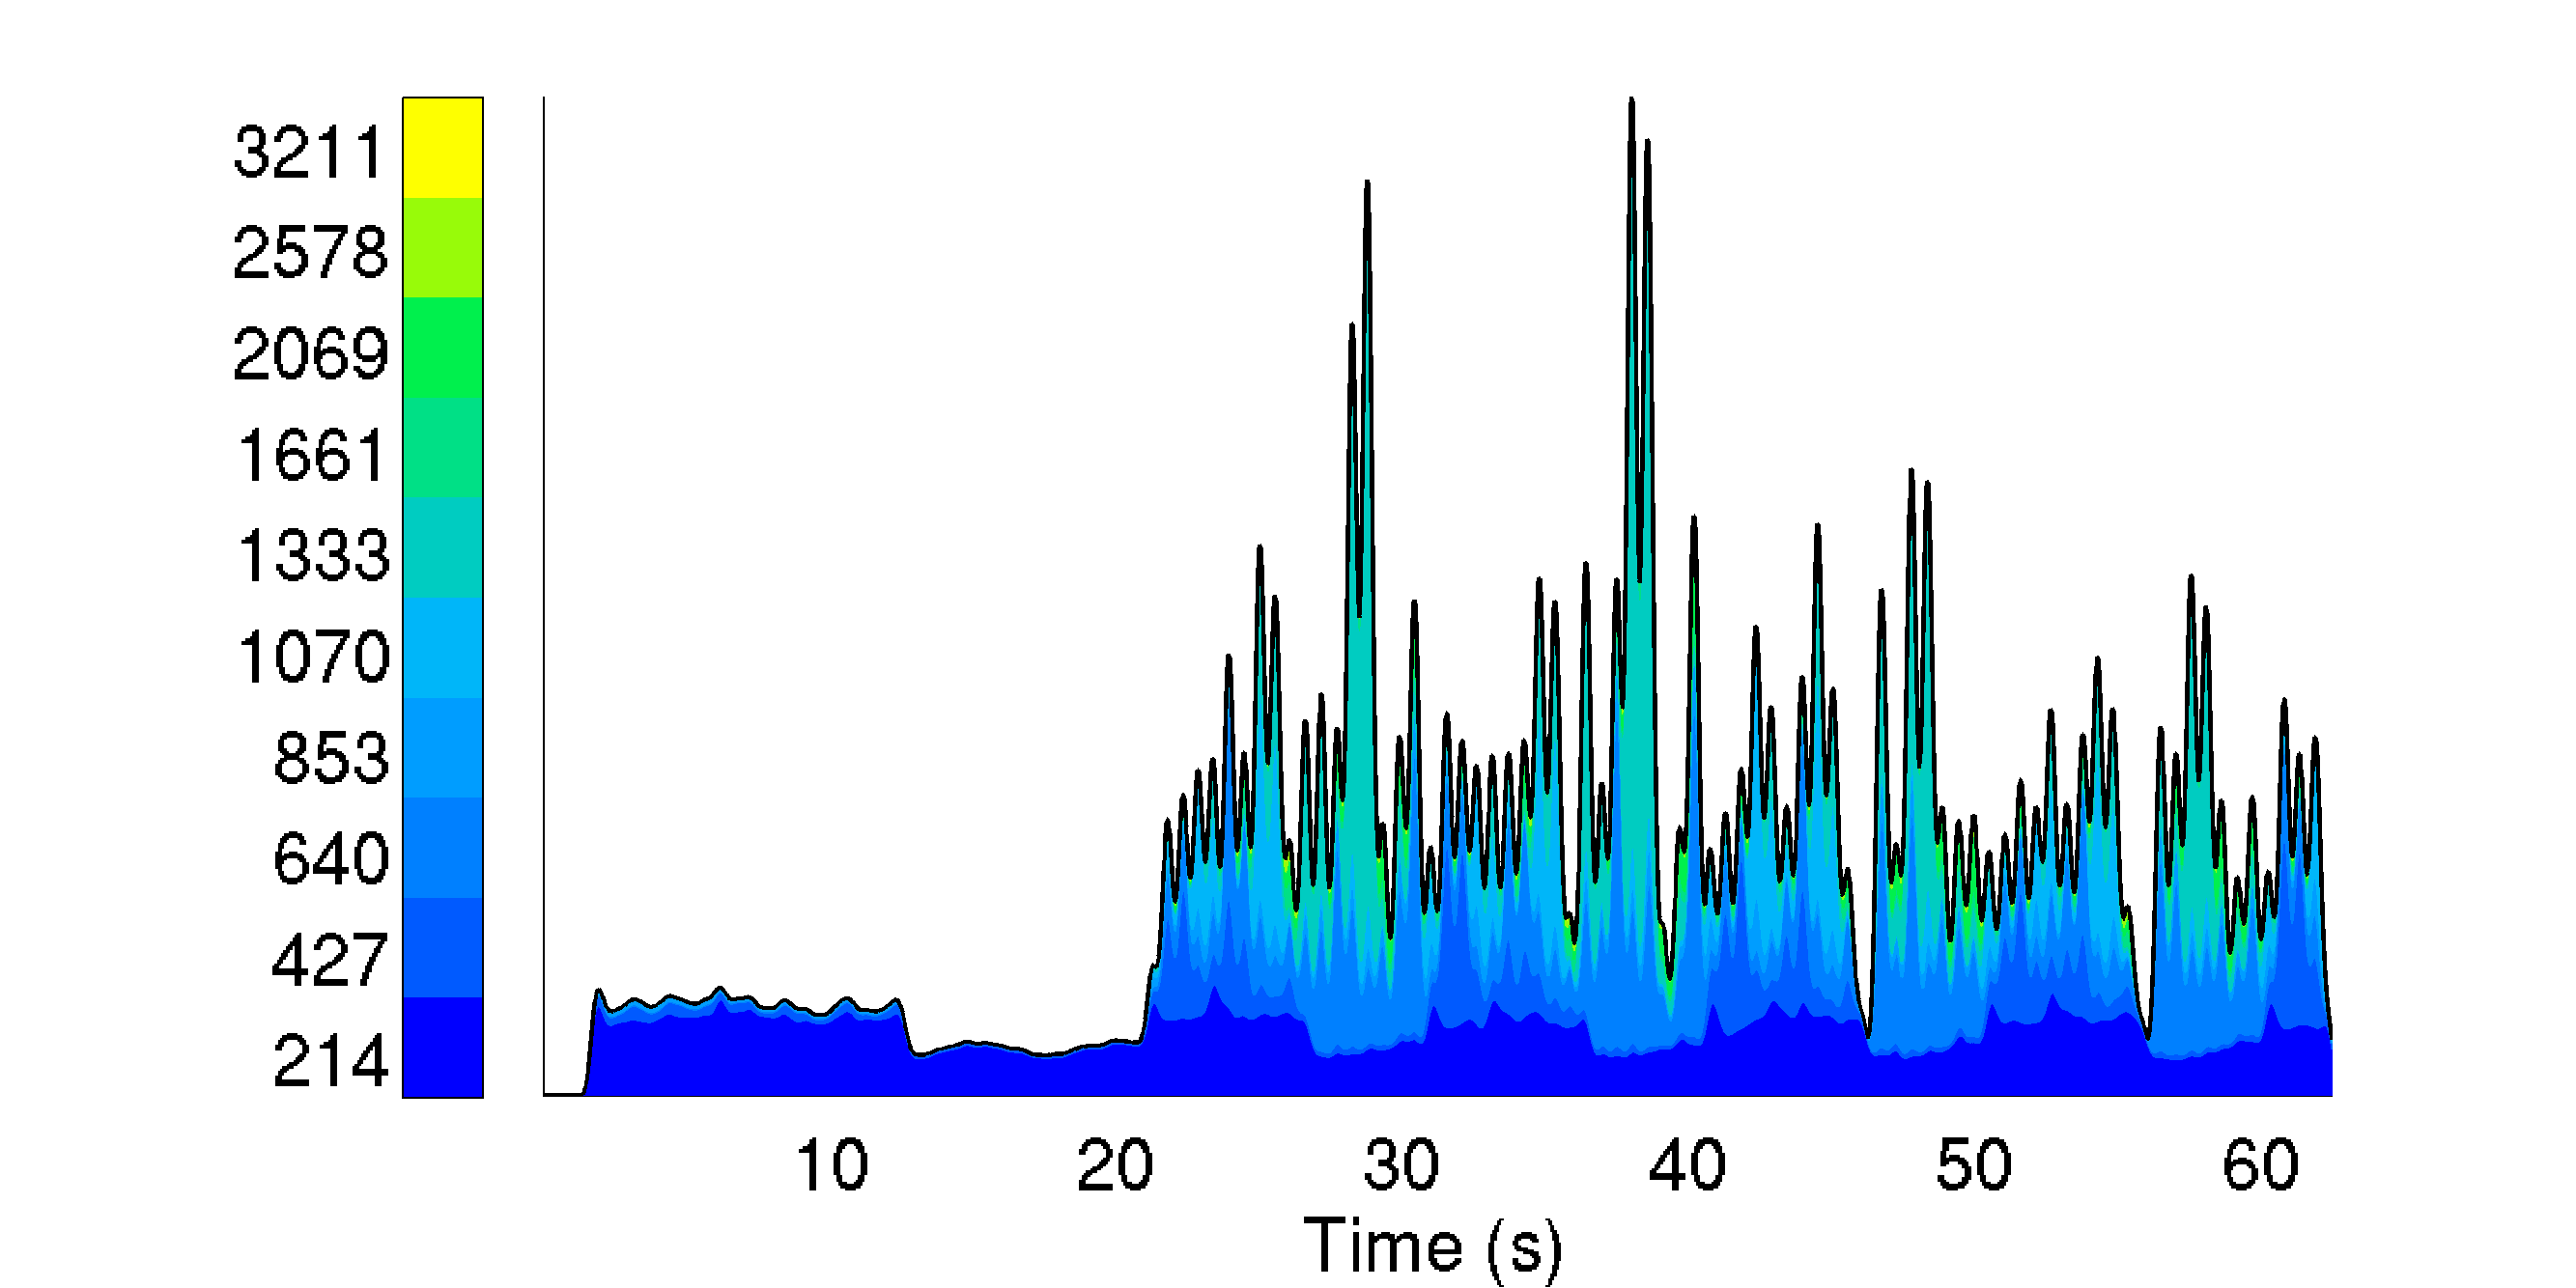
\includegraphics[width=\textwidth]{einstein_spack}
\caption{SPectral stACK (SPACK) display of the musical piece "Einstein on the beach".}
\label{fig:einstein}
\end{figure*}


\begin{figure*}
 \centering
\begin{subfigure}[b]{.4\textwidth}
\caption{}
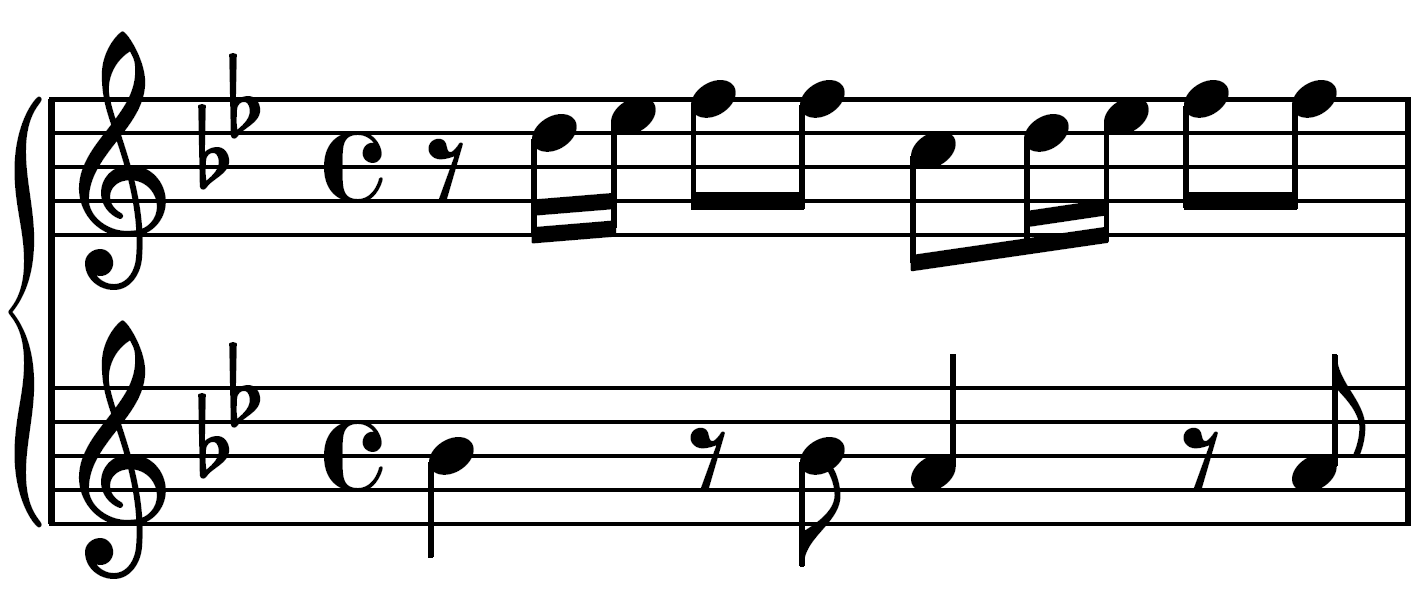
\includegraphics[width=\textwidth]{telemann}
\label{fig:telemann}
\end{subfigure}
\begin{subfigure}[b]{\textwidth}
\caption{}
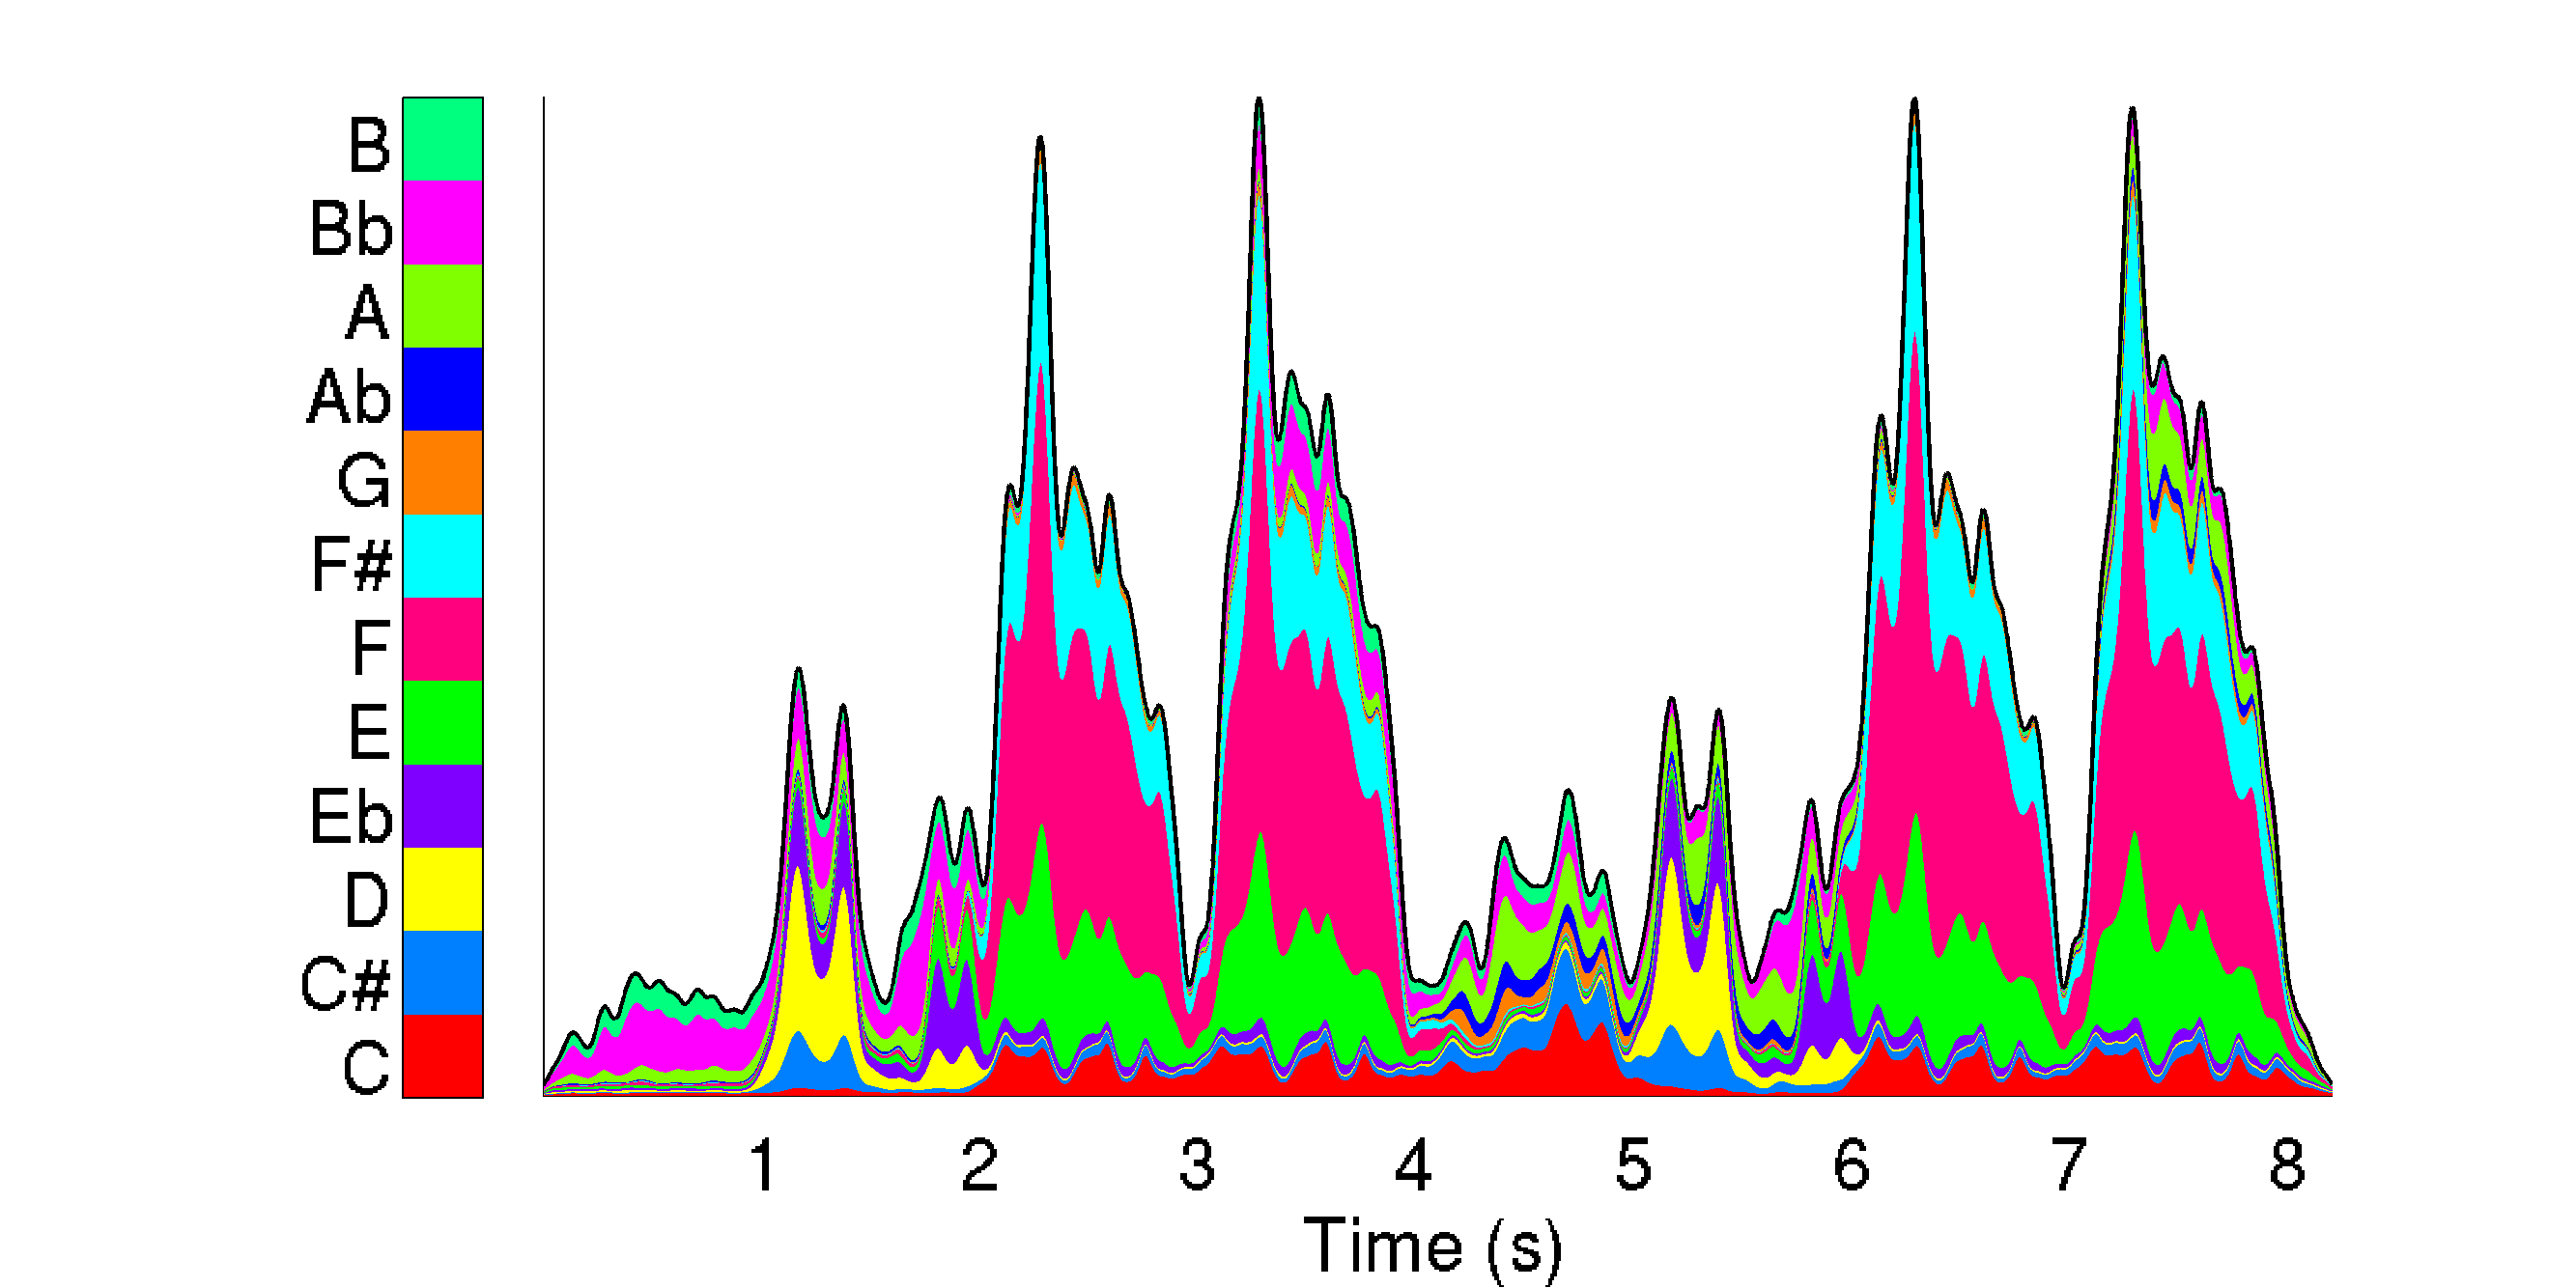
\includegraphics[width=\textwidth]{duoFluteMono_schack}
\label{fig:duoFluteMono_schack}
\end{subfigure}
\caption{Musical score (a) of the extract of a flute \textit{Duett} by George Philipp Telemann (1681-1767) and corresponding Sound CHroma stACK (SCHACK) display (b).}
\label{fig:schack}
\end{figure*}


\end{document}
